\documentclass[ngerman,12pt,listof=totoc, bibliography=totoc]{scrartcl}

% Preamble und Konfiguration laden
%-------------------------------------------------------
%-----------------------------------------------------------------------------------------------------------------------
%Abkürzungsverzeichnis
\usepackage[printonlyused]{acronym}

%Sprache festlegen auf Deutsch
\usepackage[ngerman]{babel} 

%Text ohne Bedeutung
\usepackage{blindtext}

%Quellenverzeichnis
\usepackage[natbib=true, backend=biber, style=alphabetic]{biblatex}
\addbibresource{content/bib/bibliography.bib}

%Schriftart
\usepackage{carlito}
\setmainfont{carlito}

%Kompakte Listen
\usepackage{paralist, tabularx}

%Zeichen
\usepackage{pifont}
\newcommand{\ja}{\ding{51}}
\newcommand{\nein}{\ding{55}}

%Fortgeschrittene Funktionen für Zitate 
\usepackage{csquotes}

%Positionierung von Tabellen und Abbildungen
\usepackage{float}

%OpenType fonts können geladen werden
\usepackage{fontspec}

%Seitenränder einstellen
\usepackage[left=3.0cm, right=3.0cm, head=2.5cm, bottom=3cm]{geometry}

%Abbildungen
\usepackage{graphicx}
\graphicspath{{content/images/}}

%Verweise
\usepackage[hidelinks]{hyperref}
\usepackage{cleveref}   %cleveref muss nach hyperref geladen werden

%Header / Footer
\usepackage[headsepline,footsepline,plainfootsepline]{scrlayer-scrpage}
\renewcommand*{\sectionmarkformat}{} %lässt die Nummerierungszahl der Section aus dem Header verschwinden
\clearpairofpagestyles
\ohead{\headmark}
\automark{section}
\ofoot[\pagemark]{\pagemark}
\cfoot[\thesistitel]{\thesistitel}

%Zeilenabstand einstellen
\usepackage[onehalfspacing]{setspace}

%Bilder, Tabellen etc. nebeneinander platzieren
\usepackage{subcaption}

%Für Notizen
\usepackage[colorinlistoftodos,prependcaption]{todonotes}

% Wird gebraucht um Fehlermeldung wegzubekommen
\setlength {\marginparwidth }{2cm} 

%TODOS
\newcommand{\comingSoon}[1]{\todo[inline,linecolor=red,backgroundcolor=orange!40, bordercolor=black]{#1}}
\newcommand{\unsure}[1]{\todo[inline,linecolor=red,backgroundcolor=red!40, bordercolor=black]{#1}}
\newcommand{\change}[1]{\todo[linecolor=blue, backgroundcolor=blue!40, bordercolor=black]{#1}}
\newcommand{\info}[1]{\todo[shadow, noline,linecolor=green, backgroundcolor=green!40, bordercolor=black]{#1}}
\newcommand{\improvement}[1]{\todo[linecolor=violet,backgroundcolor=violet!40,bordercolor=black]{#1}}

%Code
\newcommand{\code}[1]{\texttt{#1}}

%Farben
\usepackage{xcolor}

%-----------------------------------------------------------------------------------------------------------------------
%Counter um die Seiten zu zählen, für römische Zahlen
\newcounter{seitenanzahl}
%Inhaltsverzeichnis ins Inhaltsverzeichnis
\setuptoc{toc}{totoc}
%-----------------------------------------------------------------------------------------------------------------------

%Namen des Autors
\newcommand{\thesisauthor}{Autor}

%Titel der Arbeit
\newcommand{\thesistitel}{PA-Titel}

%Genaue Bezeichnung der Arbeit
\newcommand{\thesistyp}{Projektarbeit XX}

%Abgabedatum der Arbeit
\newcommand{\abgabedatum}{XX.XX.XXX}

%Kursname
\newcommand{\kurs}{XXXX}

%Studiengang
\newcommand{\studiengang}{Informatik}

%Abschluss
%\newcommand{\abschluss}{Bachelor of Science}

%Name des Unternehmens
\newcommand{\unternehmen}{Unternehmensname}

%Name des Betreuers im Unternehmen
\newcommand{\unternehmensbetreuer}{XXXX}

%Standort des Unternehmens
\newcommand{\arbeitsort}{Ort}

%Name des DHBW-Betreuers
\newcommand{\dhbwbetreuer}{XXXX}

%Datum für die ehrenwörtliche Erklärung
\newcommand{\datumerklaerung}{XX.XX.XXXX}

%Ort der ehrenwörtlichen Erklärung
\newcommand{\orterklaerung}{Ort}

%Datum der Freigabe durch das Unternehmen
\newcommand{\datumfreigabe}{XX.XX.XXXX}

%Ort der Freigabe 
\newcommand{\ortfreigabe}{Ort der Freigabe}

%Datum der Unterschrift des Autors beim Sperrvermerk
\newcommand{\sperrvermerkdatumauthor}{XX.XX.XXXX}

%Datum der Unterschrift des Unternehmens beim Sperrvermerk
\newcommand{\sperrvermerkdatumunternehmen}{XX.XX.XXXX}

%Adresse des Unternehmens
\newcommand{\unternehmensadresse}{Beispiel-Adresse XX, XXXX Stadt}

%Email des Unternehmens
\newcommand{\unternehmsemail}{XXXX}

%Telefonnummer des Unternehmens
\newcommand{\unternehmenstel}{XXXX}

%Variable ob es sich um eine Studienarbeit handelt
\newif\ifseminararbeit  %Deklaration
\seminararbeitfalse     %Zuweisung des Wertes true

%Variable ob es einen Sperrvermerk gibt
\newif\ifsperrvermerk   %Deklaration
\sperrvermerkfalse       %Zuweisung des Wertes true

%Variable ob es einen DHBW-Betreuer gibt
\newif\ifdhbwbetreuer   %Deklaration
\dhbwbetreuerfalse      %Zuweisung des Wertes false

%-------------------------------------------------------

\begin{document}

\spacing{1.5}

\author{\thesisauthor}
\title{\thesistitle}
\date{\abgabedatum}
\pagestyle{plain.scrheadings}
\pagenumbering{Roman}

\thispagestyle{empty}

\vspace*{-2.5cm}

\ifseminararbeit
\else

\includegraphics[width=6cm]{Dota2Logo}
\fi
\hfill

\includegraphics[width=6cm]{logo-dhbw}
\vspace*{3cm}

\begin{center}
{\LARGE \thesistitel} \\
\vspace{0.5cm}

\ifsperrvermerk 
\textcolor{red}{\large mit Sperrvermerk\\}
\else
\vspace{2cm}
\fi

\vspace{1cm}

\textbf{\large \thesistyp}\\

%\vspace{2cm}
%für die Prüfung zum \\ 
%\abschluss \\

\vspace{2cm} 
des Studiengangs \studiengang \\
an der \\
Dualen Hochschule Baden-Württemberg Lörrach \\

\vspace{1cm}
\thesisauthor \\
\abgabedatum
\vfill

\begin{tabular}{l l}
Kurs & \kurs \\
Ausbildungsunternehmen & \unternehmen \\

\ifseminararbeit
\else
Unternehmensbetreuer & \unternehmensbetreuer \\
\fi

\ifdhbwbetreuer
Wissenschaftlicher Betreuer & \dhbwbetreuer \\
\fi

\end{tabular}
\end{center}
\addsec{Ehrenwörtliche Erklärung}
\noindent Ich versichere hiermit, dass ich meine \thesistyp{} mit dem Thema:
\begin{center}
\textbf{ \thesistitel}
\end{center}

\noindent selbstständig verfasst und keine anderen als die angegebenen Quellen und Hilfsmittel benutzt habe. Ich versichere zudem, dass die 				  eingereichte elektronische Fassung mit der gedruckten Fassung übereinstimmt.

\vspace*{1cm}
\noindent \orterklaerung, \datumerklaerung{} \\
\vspace*{1.5cm} \\
\noindent\rule{8cm}{0.5pt}\\
\thesisauthor
\vfill*

\addsec{Hinweise zum Umfang der Arbeit}

\noindent Der Textteil der vorliegenden Arbeit - beginnend mit der Einleitung bis ausschließlich Quellenverzeichnis - umfasst \pageref{seitenreinschrifft} Seiten.




\ifseminararbeit
\else
\addsec{Freigabe der Arbeit}
\noindent Die vorliegende Arbeit wurde durch das Ausbildungsunternehmen 
\unternehmen{}, inhaltlich geprüft und zur Vorlage an der DHBW Lörrach, Studiengang \kurs, freigegeben.

\vspace*{4cm}
\begin{center}
	\begin{tabular}[h]{cc}
		\noindent\rule{7cm}{0.5pt} & \noindent\rule{7cm}{0.5pt} \\
		\noindent\ortfreigabe, \datumfreigabe & \unternehmensbetreuer
 	\end{tabular}
\end{center}

\fi

\ifsperrvermerk 
\addsec{Sperrvermerk}
Der Inhalt dieser Arbeit darf weder als Ganzes noch in Auszügen Personen außerhalb des Prüfungsprozesses und des Evaluationsverfahrens zugänglich gemacht werden, sofern keine anders lautende Genehmigung der Ausbildungsstätte vorliegt.
\vspace{4cm}
\begin{center}
 \begin{tabular}[h]{cc}
   \noindent\rule{7cm}{0.5pt} & \noindent\rule{7cm}{0.5pt} \\
   \noindent\sperrvermerkdatumauthor, \thesisauthor & \sperrvermerkdatumunternehmen, \unternehmen
 \end{tabular}
\end{center}
\vspace{2cm}
\textbf{Kontakt:} \\
\unternehmen \\
\unternehmensadresse \\
\unternehmsemail \\
\unternehmenstel 

\fi

\addsec{Kurzfassung}

In dieser Projektarbeit wird die Thematik behandelt um die Untersuchung der digitalen Barrierefreiheit in Dialogen der Desktopanwendungen. Es wird geprüft, inwiefern die Umsetzbarkeit der Standards der digitalen Barrierefreiheit in Dialogen der Desktopanwendungen möglich ist. Für den Zweck werden Normen der \ac{WCAG} 2.0 bzw. der \ac{WCAG} 2.1 betrachtet. Die Richtlinien der erwähnten Normen werden anhand ihrer Erfolgskriterien ausgewertet.

Als Resultat dieser wissenschaftlichen Arbeit wird ein Katalog der in den Desktop Dialogen umsetzbaren Kriterien des Standards der digitalen Barrierefreiheit erstellt. Dieser wird dementsprechend nicht nur für den Abbau von digitalen Barrieren der aktuellen Software verwendet, sondern auch bei der Entwicklung neuer Software berücksichtigt.

Die AKG-Software besitzt als Hilfsmittel zu ihrer Software eine webbasierte Dokumentation, die jeden Dialog der Software beschreibt und alle Funktionalitäten dieses Dialogs erklärt. Nichtsdestotrotz wird die Software nicht als barrierefrei bezeichnet, falls die Dokumentation barrierefrei ist. Infolgedessen wird in dieser Arbeit nicht untersucht, ob die webbasierte Dokumentation barrierefrei ist.
\tableofcontents

\addsec{Abkürzungsverzeichnis}

%% Das Paket kann nicht automatisch sortieren
\begin{acronym}[VCS]

\acro{BITV}{Barrierefreie-Informationstechnik-Verordnung}
\acro{CAPTCHA}{Completely Automated Public Turing test to tell Computers and Humans Apart}
\acro{GUI}{Graphical User Interface}
\acro{IKT}{Informations- und Kommunikationstechnik}
\acro{TFS}{Team Foundation Server}
\acro{WAI}{Web Accessibility Initiative}
\acro{WCAG}{Web Content Accessibility Guidelines}
\acro{W3C}{World Wide Web Consortium}

\end{acronym}

\clearpage
\listoffigures
\clearpage
\listoftables
\clearpage
\setcounter{seitenanzahl}{\value{page}}
\pagenumbering{arabic}
\pagestyle{scrheadings}

%Hier kommen die eigentlichen Kapitel
%-----------------------------------------------------------
\section{Einleitung}

\subsection{Aufbau der Arbeit und methodisches Vorgehen}
Als erstes wird die digitalen Barrierefreiheit definiert und es wird auf die Nachteile fehlender Barrierefreiheit in Software eingegangen. Außerdem wird die Zielerreichung dieser Arbeit in \cref{subsec: Schaffung von Barrierefreiheit in Desktopanwendungen und Abgrenzung der Arbeit} dargestellt. Danach wird das Unternehmen und die Softwareabteilung des Unternehmens vorgestellt. Darüber hinaus werden wichtige Begriffe erklärt. Es wird auch begründet, aus welchem Grund auf die digitale Barrierefreiheit geachtet werden muss. Welche Rolle die digitale Barrierefreiheit in der Software-Entwicklung spielt und wieso zwischen Barrierefreiheit und Behindertengerecht unterschieden werden muss, wird durch Betrachtung der Ist-Zustand klar gemacht. Vom \cref{subsec:Prinzipien fuer Barrierefreiheit} bis \cref{subsec: Normen der WCAG 2.1} werden Normen der digitalen Barrierefreiheit von der "`World Wide Web Consortium"' \footnote{The World Wide Web Consortium (W3C) \cite{w3c}} sowie die Unterschiede zu den \ac{BITV} präsentiert. Schließlich werden Kriterien der Standards auf die Umsetzbarkeit in Dialogen der Desktopanwendungen hin untersucht.

\subsection{Ein Blick in die Vergangenheit der Barrierefreiheit}
Der Begriff Barrierefreiheit wurde seit den 1970er-Jahren von Menschen mit Behinderungen eingefordert und wird in Deutschland als Synonym für den englischen Bergriff \textit{Accessibility} betrachtet. Es beutet, dass Menschen mit Behinderungen den Zugang zu unterschiedlichen Infrastrukturen haben. Der Begriff Barrierefreiheit ist im Bereich der Nutzung von Gebäuden oder Verkehrsmitteln im Sinne von \textit{Zugang} wörtlich zu nehmen, da die Rede vom physischen Zugang ist. Sobald man von der Formation und der Kommunikation redet, erweitert sich der Begriff vom physikalischen Zugang zu den Inhalten, den Bedingungen und dem Verständnis.\footnote{Accessibility über Desktopanwendungen hinaus–Barrierefreiheit \cite{buhler2017accessibility}} Der Begriff Barrierefreiheit bekam im Jahr 2002 eine moderne gesetzliche Definition, die im Jahr 2016 angepasst wurde: "`Barrierefrei sind bauliche und sonstige Anlagen, Verkehrsmittel, technische Gebrauchsgegenstände, Systeme der Informationsverarbeitung, akustische und visuelle Informationsquellen und Kommunikationseinrichtungen sowie andere gestaltete Lebensbereiche, wenn sie für Menschen mit Behinderungen in der allgemein üblichen Weise, ohne besondere Erschwernis und grundsätzlich ohne fremde Hilfe auffindbar, zugänglich und nutzbar sind."'\footnote{Vgl. Accessibility über Desktopanwendungen hinaus–Barrierefreiheit S. 501 \cite{buhler2017accessibility}}

Diese Definition betrachtete die Nutzbarkeit als Hauptanliegen, jedoch die Wandlung zur Informations- und Wissensgesellschaft war nicht mehr zu ignorieren und damit kam der Anwendungsbereich der \ac{IKT} in das Blickfeld. Das Nichtnutzen dieser alternativen Zugangsmöglichkeiten hat Menschen mit Behinderungen, die nicht online gehen können getroffen. Diese Zielgruppe war benachteiligt oder sogar ausgeschlossen. Fügt man nun die \ac{IKT} zu der vorherigen Definition hinzu, wird der Zusammenhang mit der \textit{Zugänglichkeit} unmittelbar deutlich.\footnote{Accessibility über Desktopanwendungen hinaus–Barrierefreiheit \cite{buhler2017accessibility}}

\subsection{Die Bedeutung der digitalen Barrierefreiheit}
\label{subsec: Die Bedeutung der digitalen Barrierefreiheit}

Digitale Barrierefreiheit bedeutet, dass Menschen das Internet nutzen können, dessen Inhalte wahrnehmen, verstehen, navigieren und mit ihm integrieren können. In dieser Hinsicht kommen Menschen mit Behinderungen stärker in den Fokus.\footnote{Gesellschaft für digitale Bildung \cite{GFDB}} "`Laut der Aktion Mensch-Studie nutzen Menschen mit Behinderung das Internet öfter als Menschen ohne Behinderung. Elektronische Interaktionen sind demnach von besonderer Bedeutung, weil sie Zugang zu bestimmten Angeboten überhaupt erst ermöglichen."'\footnote{Vgl. Gesellschaft für digitale Bildung \cite{GFDB}}. Aber unter der digitalen Barrierefreiheit betrachtet man mehr als die körperlichen Einschränkungen wie z.B. Schwerhörigkeit oder Blindheit, wie beispielsweise die fehlende Möglichkeit, einen Ton abzuspielen. Ebenso verhält es sich mit der Kontrasterkennung bestimmter Farben oder der Gestaltung der Inhalte. Außerdem sind viele digitale Angebote, die oft \textbf{exklusiv} online verfügbar sind, nur schwer zu bedienen. Anders gesagt, sie sind nicht \textit{nutzerfreundlich}. Diese Barrieren sind alles Faktoren, die für alle Menschen eine Rolle spielen und auch ganze Zielgruppen ausschließen können.\footnote{Gesellschaft für digitale Bildung \cite{GFDB}} Es ist also zu unterscheiden zwischen Barrierefreiheit und Behindertengerecht, was in \cref{subsec:Barrierefreiheit und Behindertengerecht} ausführlich erklärt ist. Um nun Barrierefreiheit in den digitalen Software zu schaffen, sind vier Prinzipien in jeder \ac{GUI} zu erfüllen. Diese sind laut \ac{WCAG} 2.0 \footnote{Web Content Accessibility Guidelines 2.0 \cite{caldwell2008web}}:

\begin{itemize}
	\item Wahrnehmbar
	\item Bedienbar
	\item Verständlich
	\item Robustheit
\end{itemize}

Auf die einzelnen Begriffe wird in \cref{subsec:Barrierefreiheit und Behindertengerecht} eingegangen.

\subsection{Fehlende Barrierefreiheit in Desktopanwendungen}
\label{subsec: Fehlende Barrierefreiheit in Desktopanwendungen}

Viele Zielgruppen werden die Software nicht nutzen können und alle anderen Nutzer haben es nicht leicht zurechtzukommen. Das sind die ersten Folgen der fehlenden Barrierefreiheit in jeder Software. "`Um die Herausforderungen an Barrierefreiheit zu verstehen, muss man sich die Diversität der Nutzerinnen und Nutzer vor dem Hintergrund der Variation der Geräte und Anwendungen vor Augen führen. Diese ist schon ohne die Berücksichtigung von Menschen mit Behinderungen sehr groß und unterscheidet sich im Hinblick auf z. B. die technische Sozialisation (,,digital native“, ,,digital illiterate“), den Bildungsgrad (Analphabetismus, akademische Bildung), die Nutzung (beruflich, die Nutzung für Information und Kommunikation, für Spiele, für Gesundheitsanwendungen) sowie die Umgebung und die Situation der Nutzung usw. Schon hier wird deutlich, dass unterschiedlichste Anforderungen berücksichtigt werden müssen, um alle Bedarfe abzudecken."'\footnote{Vgl. Accessibility über Desktopanwendungen hinaus–Barrierefreiheit S. 504 \cite{buhler2017accessibility}}

Zusammengefasst sind folgende Nachteile der digitalen Barrieren in jeder Software zu beachten:
\vspace{1em}

\begin{itemize}
	\item Es wird keine größere Reichweite erreicht
	\item Weniger Performance, denn nicht alle Menschen können die Software nutzen
	\item Weniger Erfolg, denn Menschen, die die Software regelmäßig verwenden, werden diese auch nicht weiter empfehlen, wenn sie selber Schwierigkeiten damit haben
\end{itemize}

\subsection{Schaffung von Barrierefreiheit in Desktopanwendungen und Abgrenzung der Arbeit}
\label{subsec: Schaffung von Barrierefreiheit in Desktopanwendungen und Abgrenzung der Arbeit}

Ziel dieser Arbeit ist das Untersuchen der Machbarkeit der Schaffung von digitaler Barrierefreiheit in der aktuellen Software sowie Regeln dafür festzulegen, wie in jeder Software der AKG Software Consulting GmbH digitale Barrierefreiheit umgesetzt werden kann. Bei der Entwickelung neuer Software soll auf diese Regeln geachtet werden, um digitale Barrieren so gut wie möglich zu vermeiden. Es wird untersucht, wie man die digitale Barrierefreiheit erreicht, wofür die Normen der \ac{WCAG} 2.0 bzw. der \ac{WCAG} 2.1 in Frage kommen, die auch möglicherweise nicht komplett umsetzbar sein können. Außerdem wird auf die Vor- und Nachteile, die einem Entwickler begegnen werden, eingegangen. Zu der aktueller Software bietet das Unternehmen eine Dokumentation an, die jedes Dialog der Software beschreibt. Dazu gehört eine Beschreibung von der Struktur, inhaltlichen Informationen, Fachbegriffen usw.. Diese Dokumentation ist webbasiert und wird bei der Untersuchung der Barrierefreiheit in dieser Projektarbeit nicht betrachtet.
\section{Grundlagen}
Die folgenden Unterabschnitte sind essentielle Bausteine zum Verstehen dieser Arbeit.

\subsection{AKG Software Consulting GmbH}
Das Unternehmen AKG ist ein Software-Entwicklungs-Unternehmen. Im Unternehmen wird Software für die Straßenplanung hergestellt. Die hergestellte Software umfasst ein breites Spektrum, von der Straßenplanung bis zur Kostenberechnung. Die Software besteht aus vielen Modulen, die jeweils einen Fachbereich behandeln und basiert auf
einer CAD-Plattform. Als Basis kommen drei unterschiedliche Plattformen zum Einsatz. Bei AKG wird die Software kontinuierlich weiterentwickelt und in halbjährlichen
Software-Versionen für die Kunden veröffentlicht. In den Software-Versionen werden jeweils wichtige Korrekturen für Software-Fehler und neue Funktionalitäten eingeführt. Die Entwicklung der Software wird in den sieben Firmensitzen von AKG durchgeführt. Neben dem Hauptfirmensitz in Heitersheim gibt es weitere Firmensitze in Berlin, Wien, Köln, Hamburg, Halle und Landquart. Für den Software-Entwicklungsprozess sind mehrere Abteilungen notwendig, die es in jedem Firmensitz gibt. Dazu gehören die Entwicklungsabteilung, die Qualitätssicherungsabteilung und die Support-Abteilung. Zur Verwaltung der Software-Entwicklung wird ein \ac{TFS} standortübergreifend verwendet. Im \ac{TFS} werden die Software Versionen, der Quellcode, die Aufgaben und weitere Aspekte der Software-Entwicklung verwaltet. Zur Kommunikation verwenden die Mitarbeiter standortübergreifend die Anwendung „Microsoft Teams“ (MS Teams). In den neusten Software-Versionen sind trotz aller Maßnahmen immer einige Software-Fehler vorhanden. Diese Software-Fehler können von den Kunden bemerkt und an die Mitarbeiter von AKG gemeldet werden. Die gemeldeten Software-Fehler werden anschließend von den Mitarbeitern von AKG behoben und in der nächsten Software-Version für die Kunden veröffentlicht. Das Erfassen der Fehler läuft über die Support-Abteilung bei AKG ab. Die Kunden können über ein Ticketsystem Software-Fehler in Form von Tickets an die Support-Abteilung melden. Die Mitarbeiter der Support-Abteilung kümmern sich um die weitere Bearbeitung der Tickets. Entweder wird das Ticket durch die Mitarbeiter der Support-Abteilung gelöst oder an die Entwicklungsabteilung weitergeleitet, damit das Ticket in der Software behoben werden kann.

\subsubsection{Abteilungsvorstellung}
In der Entwicklungsabteilung beschäftigen sich die Mitarbeiter damit, die Software-Fehler zu korrigieren und neue Funktionalitäten umzusetzen. Jeder Mitarbeiter ist dabei für bestimmte Module in der Software zuständig. Pro Modul können mehrere Mitarbeiter und jeder Mitarbeiter kann für mehrere Module zuständig sein. Die Mitarbeiter der Qualitätssicherungsabteilung sind dafür zuständig, die umgesetzten Änderungen der Entwicklungsabteilung in der Software zu überprüfen. Jede Änderung wird durch einen Mitarbeiter aus der Qualitätssicherungsabteilung geprüft, bevor die Änderung an die Kunden veröffentlicht werden kann. Bei fehlerhafter Umsetzung einer Änderung werden die Entwickler zur Korrektur der Änderung aufgefordert.

\subsection{Definitionen}
Die folgende Definitionen dienen zur besseren Verständnis bestimmter Begriffe dieser Arbeit.

\begin{description}
	\item[CAPTCHA]\hfill \\
	\begin{figure}[h]
		\begin{minipage}{0.5\textwidth}
			Steht für "`Completely Automated Public Turing test to tell Computers and Humans Apart"' im Deutschen ein vollständig automatisierter öffentlicher
			Turing-Test, um einen Menschen vom Computer zu unterscheiden.\footnote{Captcha security: A case study \cite{yan2009captcha}}
			% \caption{Der Text}
			% \label{Text}
		\end{minipage}
		\hfill
		\begin{minipage}{0.4\textwidth}
			% \textwidth bezieht sich nun auf die Minipage
			
\includegraphics[width=\textwidth]{CAPTCHA.png}
			\caption{Beispiel-CAPTCHA. \\Quelle: \cite{yan2009captcha}}
			%\label{Bild} 
		\end{minipage}
		% \caption{noch eine Caption für die Figur}
	\end{figure}

	\item[Informations- und Kommunikationstechnik]\hfill \\
	\ac{IKT}: Der Begriff entstand zur Beginn der 90er Jahre des vorherigen Jahrhunderts. Bereits in den 1990er war man der Auffassung, dass beide
	Bereiche zusammenwachsen würden. Die Informationstechnologie umfasste damals die Großrechner. Die Kommunikationstechnologie hingegen beschäftigte
	sich ausschließlich mit dem Fernsprechnetz. Seit etwa 2000 wird der Begriff häufig als Oberbegriff für alles verwendet, was mit Information und Kommunikation
	zu tun hat.
	\\
	\unsure{Entweder finde die Quelle oder die Definition von einer anderen Quelle nehmen}

	\item [Erfolgskriterium]\hfill \\
	Ein Erfolgskriterium ist eine testbare Aussage, die entweder wahr oder falsch ist, wenn man sie auf konkrete Webinhalte anwendet. In dieser
	Arbeit sind die Erfolgskriterien zur Erfüllung der Barrierefreiheit der \ac{WCAG} gemeint.\footnote{Web Content Accessibility Guidelines 2.0 \cite{WCAG2.0}}

	\item[\ac{WAI}]\hfill \\	
	Die \ac{WAI} ist eine Initiative der \ac{W3C}. Die \ac{WAI} entwickelt Standards und Hilfsmitteln, die beim Verstehen und bei der Umsetzung 
	der Barrierefreiheit helfen.\footnote{The World Wide Web Consortium (W3C) \cite{w3c}}

	\item[\ac{W3C}]\hfill \\
	Das \ac{W3C} ist eine internationale Community, die die Standards entwickelt, um das langfristige Wachstum des Web 
	sicherzustellen.\footnote{The World Wide Web Consortium (W3C) \cite{w3c}}
	
	\item[Audiodeskription]\hfill \\
	Audiodeskription ist eine zur Tonspur zusätzlich hinzugefügte Schilderung, um visuelle Details zu beschreiben, die allein durch die Haupt-Tonspur 
	nicht verständlich sind.\footnote{Web Content Accessibility Guidelines 2.0 \cite{WCAG2.0}}
	
	\item[Erweiterte Audiodeskription]\hfill \\
	Die erweiterte Audiodeskription wird zur audiovisuellen Inhalten hinzugefügt, indem das Video angehalten wird. Diese Zeit wird verwendet, 
	um eine zusätzliche Audiodeskription hinzuzufügen. Eine erweiterte Audiodeskription wird nur dann benutzt, wenn der Sinn des Videos ohne diese verloren geht und wenn 
	die Pausen zwischen den Schilderungen zu kurz sind, so dass die normalen Audiodeskription nicht den Sinn des Inhaltes vermitteln 
	können.\footnote{Web Content Accessibility Guidelines 2.0 \cite{WCAG2.0}}
	
	\item[Synchronisierte Medien]\hfill \\
	"`Audio oder Video, synchronisiert mit einem anderen Format für die Präsentation von Informationen und/oder mit zeitbasierten interaktiven 
	Komponenten, es sei denn, das Medium ist eine Medienalternative für Text, die als solche deutlich gekennzeichnet 
	ist."'\footnote{Web Content Accessibility Guidelines 2.0 \cite{WCAG2.0}}
	
	\item[Durch Software bestimmbar]\hfill \\
	Die vom Autor gelieferten Daten sollten so bereitgestellt werden, dass Benutzeragenten und assistierende Techniken diese Daten entnehmen können und in verschiedenen
	Formen präsentieren können.\footnote{Web Content Accessibility Guidelines 2.0 \cite{WCAG2.0}}
	
\end{description}

\subsection{Grundlagen der verwendeten Methoden}
\comingSoon{Falls noch andere Methoden kommen, dann als Unterabschnitt ausführlich und abstrakt erklären}

\subsubsection{Nutzwertanalyse}

Ist ein qualitatives Verfahren der Entscheidungstheorie. Es geht um die Beurteilung der Effektivität durch Bewertung von Alternativen/Varianten über gewichtete Zieldimensionen und Nutzeneinstufung. Die jeweiligen Beiträge werden zur Erreichung des Ziels quantifiziert. Bei einer Nutzwertanalyse werden alle Kriterien, egal ob sie monetär bewertbar sind oder nicht, gleich behandelt, da sie in ein Punktsystem umgerechnet werden. Es besteht hohe Flexibilität als Vorteil.\footnote{Nutzwertanalyse, Dr. Kristina Birn \cite{Dr.KB-Projektmanagment}}

Alle Zielkriterien werden in einem kreativen Prozess bearbeitet und ausgewählt. Die Kriterien müssen der Anforderung gerecht werden, damit sichergestellt wird, dass sie auch zur Problemlösung beitragen. Jedes Kriterium muss dazu beitragen, dass alle Kriterien insgesamt das Gesamtproblem lösen. Zudem muss jedes Kriterium bewertbar sein, d.h. das sachliche oder fachliche Hintergrundwissen, um das Kriterium bewerten zu können, muss vorhanden sein. Darüber hinaus muss ein Kriterium eine Relevanz in Bezug auf die Bewertung der Alternativen aufweisen und es muss reproduzierbar sein, d.h. die Bewertung des Kriteriums sollte zu jeder Zeit gleich ausfallen. Schließlich müssen alle Kriterien gewichtet werden und die Summe aller Gewichtungen muss 100\% ergeben. Dafür werden die Wichtigkeiten der einzelnen Kriterien auf das gesamte Problem festgestellt. Das kann mittels eines Paar-Vergleichs erfolgen.\footnote{Nutzwertanalysen in Marketing und Vertrieb \cite{kuhnapfel2014nutzwertanalysen}}

In dieser Projektarbeit wird die Nutzwertanalyse eingesetzt, um zu entscheiden, welche Software-Anforderungen der digitalen Barrierefreiheit in den Desktopanwendungen der AKG Software Consulting GmbH umsetzbar sind. Jede Anforderung bekommt eine Bewertung in Bezug auf die Erfüllung des Kriteriums auf einer Skala von 0 bis 10. Diese Bewertung wird mit der Gewichtung multipliziert, um den Punktwert zu erhalten. Jede Anforderung, die einen bestimmten Punktwert erreicht, wird angenommen und umgesetzt. \comingSoon{Hier den genauen Punkt erwähnen, den eine Anforderung erreichen soll, um als umsetzbar zu zeichnen}

Eine exemplarische Nutzwertanalyse ist in \cref{table:Beispielhafte Nutzwertanalyse} dargestellt.\footnote{Eigene Darstellung}

\begin{table}[H]
\caption[Beispielhafte Nutzwertanalyse]{Beispielhafte Nutzwertanalyse}
\vspace{0,1cm}
\begin{tabular}{cc|c|c|c|c|c|c|}
	\cline{3-8}
	& & \multicolumn{2}{c|}{\textbf{Anforderung 1}} & \multicolumn{2}{c|}{\textbf{Anforderung 2}} & \multicolumn{2}{c|}{\textbf{Anforderung 3}} \\ \hline
	\multicolumn{1}{|l|}{\textbf{Kriterium}} & \textbf{Gewichtung} & \textbf{B} & \textbf{PW} & \textbf{B} & \textbf{PW} & \textbf{B} & \textbf{PW} \\ \hline
	\multicolumn{1}{|l|}{\textbf{Kriterium 1}} & 60\%  & 4 & 2,4 & 2 & 1,2 & 3  & 1,8 \\ \hline
	\multicolumn{1}{|l|}{\textbf{Kriterium 2}} & 30\%  & 7 & 2,1 & 9 & 2,8 & 5  & 1,5 \\ \hline
	\multicolumn{1}{|l|}{\textbf{Kriterium 3}} & 10\%  & 3 & 0,3 & 1 & 0,1 & 10 & 1   \\ \hline
	\multicolumn{1}{|c|}{\textbf{Summe}}       & 100\% &   & 4,8 &   & 4,1 &    & 4,3 \\ \cline{1-2} \cline{4-4} \cline{6-6} \cline{8-8} 
\end{tabular}
\label{table:Beispielhafte Nutzwertanalyse}
\end{table}

\subsection{Motivation}

Im Jahr 2019 lebten in Deutschland 7,9 Millionen schwerbehinderte Menschen. "`Körperliche Behinderungen hatten 58\% der schwerbehinderten Menschen: Bei 25\% waren die inneren Organe beziehungsweise Organsysteme betroffen. Bei 11\% waren Arme und/oder Beine in ihrer Funktion eingeschränkt, bei weiteren 10\% Wirbelsäule und Rumpf. In 4\% der Fälle lag Blindheit beziehungsweise eine Sehbehinderung vor. Ebenfalls 4\% litten unter Schwerhörigkeit, Gleichgewichts- oder Sprachstörungen. Der Verlust einer oder beider Brüste war bei 2\% Grund für die Schwerbehinderung."' \footnote{Destatis. Statistisched Bundesamt \cite{DESTATIS}}

Diese Menschen können an der digitalen Welt nicht teilhaben, da sie auf digitale Barrierefreiheit angewiesen sind. Andere haben es schwer, denn die digitalen Barrieren nutzen keinem. Jeder wird sich über Software, mit der man problemlos klarkommen kann, freuen. Demzufolge ist der Abbau der digitalen Barrieren für alle gut. Kurzgefasst ist die Barrierefreiheit für Menschen mit Behinderungen ein Muss, sonst können sie die digitale Software gar nicht nutzen. Ältere Menschen und Menschen, die beispielsweise nicht gut sehen, lesen oder sich konzentrieren können, profitieren von barrierefreier Software. Fachleute sprechen in diesem Zusammenhang von einer "`Usability"' im Deutschen "`Benutzerfreundlichkeit"' \footnote{Bayerische Staatsregierung \cite{BS}}

Nun betrachten wir die Tatsache aus politischer Sicht: Wenn immer wieder mehr Informationen und Dienste über die neue Medien angeboten werden, dann besteht die Gefahr, dass viele digitale Dienste nicht für alle Bevölkerungsgruppen gleichermaßen zugänglich und nutzbar sind.\footnote{Das eInclusion EU Projekt--Politik zur digitalen Integration und Barrierefreiheit in Europa \cite{redingeinclusion}}
\section{Analyse des Ist-Zustandes der Barrierefreiheit der Desktopanwendungen}

\subsection{Barrierefreiheit in der Software-Entwicklung}
Blinde Menschen können keine Computermaus bedienen, d.h. dass die Software komplett per Tastatur bedienbar sein soll. Ein weiterer Grund, wieso Softwareunternehmen sich ebenfalls um digitale Barrierefreiheit kümmern sollten. Es ist eine harte Anforderung an Softwareentwickler, da es bezüglich des erwähnten Beispiels immer üblich war, die Software per Maus zu bedienen. Davon profitieren aber in dem Fall nicht nur Menschen mit Behinderungen. Funktioniert die Maus nicht mehr, so kann die Arbeit mit der Tastatur weitergehen. Programme, die eine Vorlesesoftware anbieten, können nur dann die graphische Oberfläche vorlesen, wenn sie mit Texten beschrieben wurde. Sogar Bilder sind davon betroffen. Ist die Oberfläche nicht gut beschriftet, so kann ein blinder Mensch oder auch Menschen mit Sehschwierigkeiten nichts erkennen. Für Menschen mit Seheinschränkungen ist beispielsweise ein Textcursor, der lediglich als senkrechter Strich im Eingabefeld dargestellt ist, nur schwer zu erkennen. Tastenkombinationen sind auch Barrieren, die für Menschen, die behinderungsbedingt nur eine Hand für das Bedienen der Software einsetzen können, die man durch die Individualisierbarkeit dieser Tastenkombinationen vermeiden kann. Individualisierbarkeit ist auch ein Begriff für Menschen mit Farbfehlsichtigkeit. Softwareunternehmen sollten die Möglichkeit anbieten, die Farben innerhalb der Software zu ändern. Da nicht jedes Unternehmen seine Software auf digitale Barrierefreiheit testet, haben Menschen mit Behinderungen sehr geringe Auswahlmöglichkeiten.\footnote{PC Welt von IDG \cite{PcWelt}}

\subsection{Barrierefreiheit und Behindertengerecht}
\label{subsec:Barrierefreiheit und Behindertengerecht}
Häufig wird das Thema Barrierefreiheit so verstanden, dass es nur bestimmte Zielgruppen betrifft. Der Grund dafür ist, dass das Thema häufig mit Erkrankungen oder Unfällen verbunden wird, die einer offiziellen ärztlichen Diagnose bedürfen. In der Tat haben viel mehr Menschen ein Bedürfnis nach barrierefreier Software, als es ihnen selbst bewusst ist. In diesem Zusammenhang stellt sich unter anderem die Frage, Warum jeder digitale Barrierefreiheit braucht. Oftmals könnten Situationen jemanden einschränken, diese Situationen erfordern barrierefreien Zugang. Was einem nach dem letzten Satz sofort einfällt, sind Menschen mit Behinderungen, jedoch ist hier die Rede von jeder Einschränkung, selbst wenn sie nicht als Behinderung bezeichnet ist. Die \cref{fig:Beispielhafte Einschränkungen} zeigt diverse Einschränkungen, die nicht als Behinderungen zählen.\footnote{Katrin Borecki Usability Engineer, MACH AG \cite{mach}}

\begin{figure}[H]
	\centering
	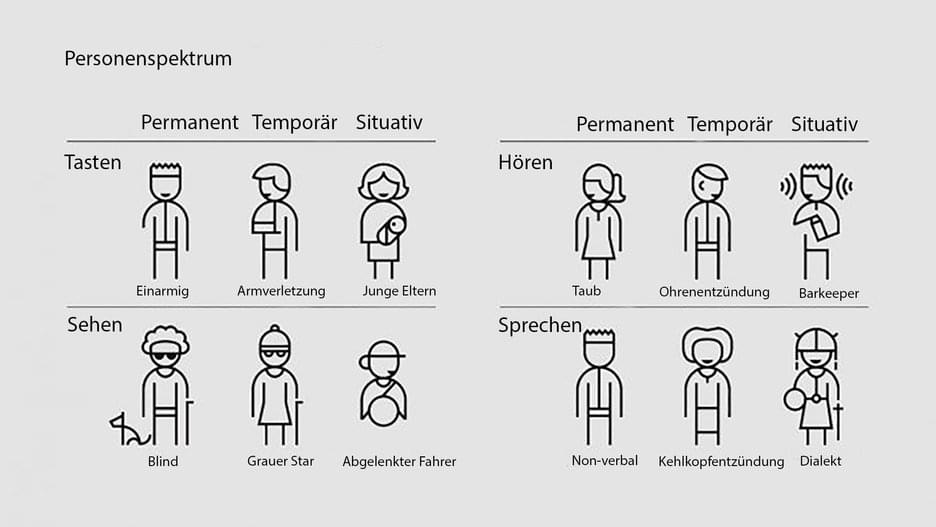
\includegraphics[width=1.0\textwidth]{Barrierefreiheit_personenspektrum}
	\caption[Personen mit verschiedenen Einschränkungen: Permanent, temporär und situativ]{Personen mit verschiedenen Einschränkungen: Permanent, temporär und situativ. 
	 Quelle: \cite{mach}}
	\label{fig:Beispielhafte Einschränkungen}
\end{figure}

Des Weiteren fühlen sich viele ältere Menschen nicht behindert. Sie stellen jedoch fest, dass für sie die Schriften kleiner sind, der Kontrast geringer ist oder der Ton weniger laut ist als früher.\footnote{Ansatz zur Behebung von digitalen Barrieren \cite{giorgashvili2020nutzerzentrierter}}

\subsection{Prinzipien für digitale Barrierefreiheit}
\label{subsec:Prinzipien fuer Barrierefreiheit}

Sowohl die Normen der \ac{WCAG} 2.0 bzw. die \ac{WCAG} 2.1 als auch die \ac{BITV} 2.0 sind so aufgebaut, dass jeder Richtlinie dieser Normen eines der vier Prinzipien zugewiesen wird. Die vier Prinzipien stellen die Grundlagen der digitalen Barrierefreiheit dar und diese sind:

\begin{description}
	\item [Wahrnehmbar]\hfill \\
	Es geht darum, dass Informationen und Bestandteile einer \ac{GUI} den Benutzern so präsentiert werden, dass Benutzer sie wahrnehmen 
	können.\footnote{Web Content Accessibility Guidelines 2.0 \cite{WCAG2.0}}
	
	Ein Beispiel für die Wahrnehmung von Inhalten ist das Kontrastverhältnis zwischen der Inhaltsfarbe und der Hintergrundfarbe. Das betrifft alle 
	mögliche Elemente der \ac{GUI} außer Logos und beiläufigen Texten. Ein praktisches Beispiel zeigt die \cref{fig:Contrast ratio}:\footnote{Web Accessibility 
	Initiative \cite{WAI}}
	
	\begin{figure}[H]
		\centering
		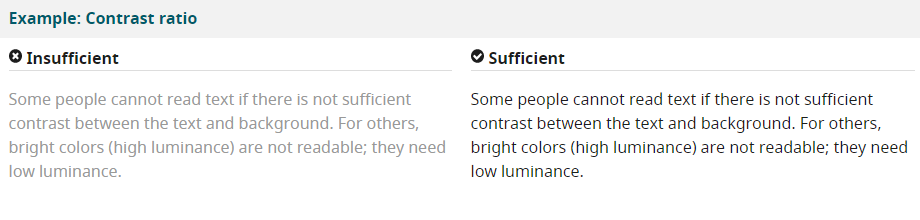
\includegraphics[width=1.0\textwidth]{Contrast ratio}
		\caption[Contrast ratio]{Contrast ratio \\Quelle: \cite{WAI}}
		\label{fig:Contrast ratio}
	\end{figure}
	
	Ein anderes Beispiel ist das ausschließliche Verwenden von Farben. Bestimmte Zielgruppen können den angebotenen Inhalt gar nicht wahrnehmen. Die 
	\cref{fig:using color alone} veranschaulicht das erwähnte Beispiel:\footnote{Web Accessibility Initiative \cite{WAI}}
	
	\begin{figure}[H]
		\centering
		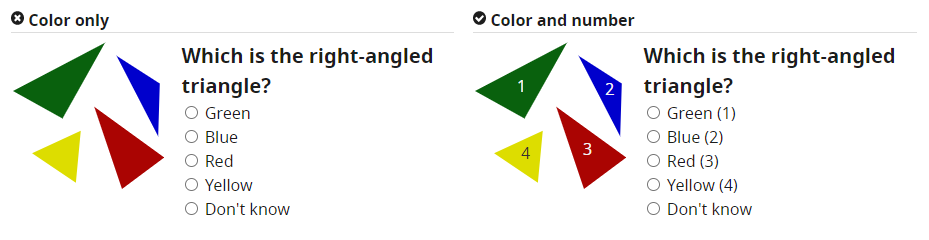
\includegraphics[width=1.0\textwidth]{Farben}
		\caption[Using color alone]{Using color alone \\Quelle: \cite{WAI}}
		\label{fig:using color alone}
	\end{figure}
	
	\item [Bedienbar]\hfill \\
	Alle Bestandteile der \ac{GUI} sowie die Navigation in dieser \ac{GUI} müssen bedienbar sein.\footnote{Web Content Accessibility Guidelines 2.0 \cite{WCAG2.0}}
	
	Beispiele für die Bestandteile der \ac{GUI} sind Links, Buttons und alle anderen interaktiven Inhalte, die z.B. den Fokus von mehreren Eingabemethoden erhalten 
	können. Diese können z.B. je nach Eingabemethode unterschiedliche Zustände bekommen, wie in \cref{fig:Ein Stile für verschiedene Linkszustände} dargestellt 
	ist:\footnote{Web Accessibility Initiative \cite{WAI}}
	
	\begin{figure}[H]
		\centering
		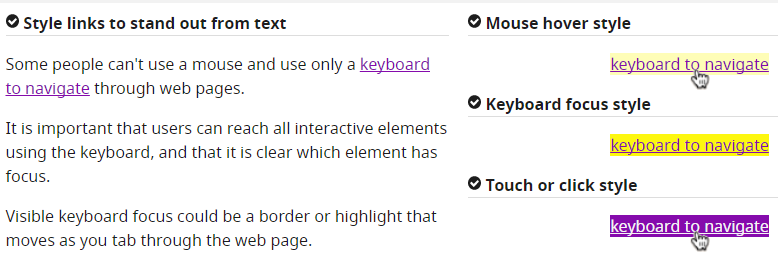
\includegraphics[width=1.0\textwidth]{Unique styles for different link states}
		\caption[Ein Stil für verschiedene Linkzustände]{Ein Stile für verschiedene Linkszustände \\Quelle: \cite{WAI}}
		\label{fig:Ein Stile für verschiedene Linkszustände}
	\end{figure}
	
	\item [Verständlich]\hfill \\
	Informationen und Bedienung der \ac{GUI} müssen den Benutzern in einer verständlichen Form präsentiert 
	werden.\footnote{Web Content Accessibility Guidelines 2.0 \cite{WCAG2.0}}
	
	Unverständliche Informationen bringen niemanden weiter. Wird beispielsweise etwas vom Nutzer verlangt oder dem Nutzer unterläuft ein Fehler, muss dem Nutzer ein entsprechendes 
	Feedback geliefert werden, so dass dieser nicht selbst nach dem Fehler suchen muss. Ein sehr bekannter Anwendungsfall, der einem regelmäßig begegnet, 
	ist die digitale Formularübermittlung. Bei einer fehlerhaften Benutzereingabe sucht der Benutzer lange nach dem Fehler, außer der Benutzer erhält entsprechendes 
	Feedback, das den Fehler und den Standort des Fehlers beschreibt. Die \cref{fig:Using error list} zeigt das erwähnte Beispiel:\footnote{Web Accessibility Initiative \cite{WAI}}
	
	\begin{figure}[H]
		\centering
		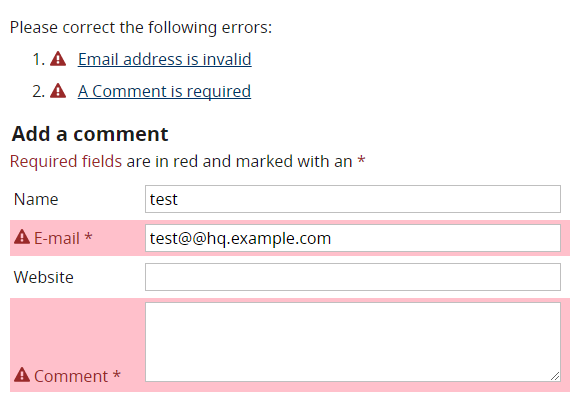
\includegraphics[width=1.0\textwidth]{Using error list}
		\caption[Verwendung von Fehlerliste, Symbol und Hintergrundfarbe, um Fehler zu markieren]{Verwendung von Fehlerliste, Symbol
		 und Hintergrundfarbe, um Fehler zu markieren. Quelle: \cite{WAI}}
		\label{fig:Using error list}
	\end{figure}
	
	\item [Robust]\hfill \\
	"`Inhalte müssen robust genug sein, damit sie zuverlässig von einer großen Auswahl an Benutzeragenten einschließlich assistierender Techniken 
	interpretiert werden können"'.\footnote{Web Content Accessibility Guidelines 2.0 \cite{WCAG2.0}}
	
	Um es überhaupt zu ermöglichen, dass z.B. assistierende Techniken funktionieren, müssen Komponenten der \ac{GUI} durch einen guten Namen, der beschreibt, was die Komponente
	ist/macht, versehen werden. Außerdem müssen Programmierer die richtigen Komponenten nehmen. Beispielsweise verhindert die Verwendung eines Bilds als Button die Verwendung 
	der assistierenden Techniken. Der folgende \textit{HTML-Code} verdeutlicht, was genau gemeint ist:
	
	Das Verwenden eines Bilds als Button:
	
	{\color{blue}
	\begin{verbatim}
		<img src="go.gif" onclick="goTo();" />
	\end{verbatim}}
	
	Stattdessen das Input-Element verwenden:
	
	{\color{blue}
	\begin{verbatim}
		<input type="button" value="go" name="Nächste_Seite_Button" />
	\end{verbatim}}
	
\end{description}

Unter den vier Prinzipien befinden sich die Richtlinien, die eine bestimmte Anzahl an testbaren Erfolgskriterien enthalten. Den Aufbau der erwähnten Normen veranschaulicht die \cref{fig:Aufbau der Normen}:\footnote{Das Konzept der \ac{WCAG} 2.0 und der \ac{BITV} 2.0 \cite{AufbauDerNormen}}

\begin{figure}[H]
	\centering
	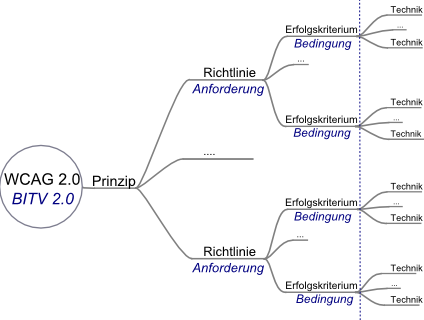
\includegraphics[width=0.8\textwidth]{Aufbau der Normen}
	\caption[Das Konzept der \ac{WCAG} 2.0 und der \ac{BITV} 2.0]{Das Konzept der \ac{WCAG} 2.0 und der \ac{BITV} 2.0 \\Quelle: \cite{AufbauDerNormen}}
	\label{fig:Aufbau der Normen}
\end{figure}

Wie in der \cref{fig:Aufbau der Normen} zu sehen ist, sind die Zweige ganz rechts Techniken. Diese sind zur Beseitigung der digitalen Barrieren von Erfolgskriterien.

\subsection{Konformitätsstufen anhand der \ac{WCAG}}
\label{subsubsec: Konformitätsstufen}
Nach den Richtlinien der \ac{WCAG} für Barrierefreiheit unterscheidet sich die Umsetzung der Anforderungen an barrierefreie Software in verschiedene Niveaus, die in drei Konformitätsstufen abgestuft sind. Diese sind:

\begin{description}
	\item [Konformitätsstufen A:] Die minimale Konformitätsstufe. Es ist ein Muss, da Menschen sonst die Inhalte nicht wahrnehmen und bedienen können. Wenn
	Erfolgskriterien der Konformitätsstufe A verletzt werden, dann ist mindestens eine Nutzergruppe von der Nutzung 
	ausgeschlossen.\footnote{Hochschule für Technik und Wirtschaft Dresden \cite{HV}}
	
	\item [Konformitätsstufen AA:] Sie ist in Europa und in Deutschland für öffentliche Stellen vorgegeben. Für eine Konformität auf dieser Stufe 
	müssen all Erfolgskriterien der Stufe \textbf{A} und der Stufe \textbf{AA} erfüllt werden. Sind die Erfolgskriterien dieser Stufe nicht umsetzbar, so
	müssen Alternativen dieser Erfolgskriterien
	zur Verfügung gestellt werden. Diese Stufe kann als angestrebte Norm bezeichnet werden, da Menschen sonst die Inhalte nur schwer wahrnehmen und bedienen 
	können.\footnote{Hochschule für Technik und Wirtschaft Dresden \cite{HV}}
	
	\item [Konformitätsstufen AAA:] Um auf diese Stufe zu kommen, müssen zuerst die ersten zwei Stufen \textbf{A} und \textbf{AA} erfüllt werden. "`Kein 
	Webauftritt wird jemals realistischerweise alle WCAG Erfolgskriterien auch der Konformitätsstufe AAA erfüllen. Nicht einmal die WAI empfiehlt, sich 
	dieses Ziel vorzunehmen. Es wird nicht empfohlen, Konformität auf Stufe AAA als allgemeine Richtlinie für komplette Websites zu fordern, da es bei manchen
	Inhalten nicht möglich ist, alle Erfolgskriterien der Stufe AAA zu erfüllen."'\footnote{Zweiter Blick \cite{ZweiterBlick}}
\end{description}

Zur besseren Vorstellung dieser Konformitätsstufen kann \cref{fig:Konformitätsstufen} \footnote{Hochschule für Technik und Wirtschaft Dresden \cite{HV}} beitragen.

\begin{figure}[H]
	\centering
	\includegraphics[width=1.0\textwidth]{Konformitätsstufen}
	\caption[Konformitätsstufen nach der \ac{BITV} 2.0]{Konformitätsstufen nach der \ac{BITV} 2.0 \\Quelle: \cite{HV}}
	\label{fig:Konformitätsstufen}
\end{figure}

\vspace{2cm}

Es bestehen jedoch Ausnahmen für Technologien, die nicht barrierefrei sind und trotzdem unter den folgenden Bedingungen eingesetzt werden dürfen:\footnote{Web Content Accessibility Guidelines 2.1 \cite{WCAG2.1}}

\begin{itemize}
	\item Falls die Inhalte parallel in einer barrierefreien Version zur Verfügung gestellt werden können.
	\item Solange die Anforderungen der Barrierefreiheit erfüllt sind, können andere Elemente die Wahrnehmung, Bedienbarkeit oder das Verständnis nicht 
	stören. Solche Elemente werden Nicht-Störende-Elemente genannt.
\end{itemize}

\subsection{Normen der \ac{WCAG} 2.0}
Die \ac{WCAG} 2.0 sind der internationale Webstandard des \ac{W3C}s zur barrierefreien Gestaltung von Internetseiten. Ab 23. September 2019 gelten die \ac{WCAG} 2.0 in der Europäischen Union für neue Webseiten und ab 23. September 2020 für bestehende Webseiten. In Deutschland wird seit 2002 die Umsetzung der \ac{WCAG} 2.0 durch die gesetzliche Verankerung in der \ac{BITV} gefördert. Die \ac{WCAG} 2.0 legen Erfolgskriterien fest, um die Konformität zu definieren.\footnote{Web Content Accessibility Guidelines 2.0 \cite{WCAG2.0}}

Es werden alle Richtlinien und ihre Erfolgskriterien der \ac{WCAG} 2.0 betrachtet, allerdings werden in \cref{subsec: Umsetzbare Kriterien} die Kriterien ausgewählt, die einen Einfluss 
auf die Desktopanwendungen haben und die in der aktuellen Software der AKG Software Consulting GmbH umsetzbar sind.

Jede Richtlinie gehört einem der vier Prinzipien der digitalen Barrierefreiheit an, was in der Aufzählung der Richtlinien im Folgenden zu sehen ist. Außerdem wird jedem Erfolgskriterium  eine Konformitätsstufe zugewiesen.

\begin{description}
	\item[Richtlinie 1.1 Textalternativen]\hfill
	\begin{itemize}
		\item \textbf{Prinzip:} Wahrnehmbar.
		\item \textbf{Allgemeine Beschreibung:} Für alle Nicht-Text-Inhalte müssen Textalternativen zur Verfügung gestellt werden, damit der Benutzer die
		präsentierte Form der Inhalte nach seinem Bedürfnis ändern kann.\footnote{Web Content Accessibility Guidelines 2.0 \cite{WCAG2.0}}
	\end{itemize}
	
	\begin{description}
		\item[Erfolgskriterium 1.1.1 Nicht-Text-Inhalt]\hfill
		\begin{itemize}
			\item \textbf{Konformitätsstufe:} A
			\item \textbf{Beschreibung:} Es müssen Mittel zum Ersetzen der Nicht-Text-Inhalte dargestellt werden können, so dass die
			Nicht-Text-Inhalte den Benutzer nicht behindern. Beispielsweise die Anpassung der Schriftgröße, die Verwendung von Symbolen oder Brailleschrift sowie die Umwandlung der Texte 
			in eine einfachere Sprache. Das sind alles Mittel, die zu Textalternativen zählen.
			Nichtsdestotrotz gibt es dafür Ausnahmen: Steuerelemente oder Eingaben durch den Benutzer, da diese einen Namen haben, der den Zweck des Element
			beschreibt. Außerdem sind Tests und Übungen von diesem Erfolgskriterium ausgenommen, da ein alternativer Text eine deskriptive Identifizierung
			des Tests oder der Übung bereitstellt und so damit der Sinn des Tests bzw. der Übung entfällt. Wenn es sich um die Vermittlung/Schaffung bestimmter
			Sinneserfahrungen handelt, kann ein Nicht-Text-Element ohne Textalternativen präsentiert werden. Darüber hinaus sind \ac{CAPTCHA} von der Regel ausgenommen,
			denn es geht darum, vom Benutzer eine Bestätigung zu verlangen, dass überhaupt eine Person und kein Computer auf den Inhalt zugreift. Allerdings gibt
			es statt der Textalternativen für das Ersetzen von \ac{CAPTCHA}s andere Ausgabeformen, die der sensorischen Wahrnehmung nutzen. Unsichtbare Elemente
			oder reine Dekoration, die ausschließlich für visuelle Formatierung verwendet wird, müssen keine Textalternativen haben, dennoch müssen
			sie so implementiert werden, dass sie von assistierender Technik ignoriert werden können.\footnote{Web Content Accessibility Guidelines 2.0 \cite{WCAG2.0}}
		\end{itemize}
	\end{description}
	
	\item[Richtlinie 1.2 Zeitbasierte Medien]\hfill
	\begin{itemize}
		\item \textbf{Prinzip:} Wahrnehmbar.
		\item \textbf{Allgemeine Beschreibung:} Es geht darum, dass Alternativen zu den zeitbasierten Medien zur Verfügung gestellt werden müssen. Davon ausgenommen sind 
		Medien, die Alternativen zum Text sind.\footnote{Web Content Accessibility Guidelines 2.0 \cite{WCAG2.0}}
	\end{itemize}
	
	\begin{description}
		\item[Erfolgskriterium 1.2.1 Reine Audio- und Videoinhalte (aufgezeichnet)]\hfill
		\begin{itemize}
			\item \textbf{Konformitätsstufe:} A
			\item \textbf{Beschreibung:} Eine Alternative für reine aufgezeichnete Audio- und Videoinhalte, die äquivalente Informationen 
			liefert, muss bereitgestellt werden.\footnote{Web Content Accessibility Guidelines 2.0 \cite{WCAG2.0}}
		\end{itemize}
			
		\item[Erfolgskriterium 1.2.2 Untertitel (aufgezeichnet)]\hfill
		\begin{itemize}
			\item \textbf{Konformitätsstufe:} A
			\item \textbf{Beschreibung:} Für alle aufgezeichneten Audioinhalte in synchronisierten Medien müssen Untertitel bereitgestellt 
			werden.\footnote{Web Content Accessibility Guidelines 2.0 \cite{WCAG2.0}}
		\end{itemize}
			
		\item[Erfolgskriterium 1.2.3 Audiodeskription (aufgezeichnet)]\hfill
		\begin{itemize}
			\item \textbf{Konformitätsstufe:} A
			\item \textbf{Beschreibung:} Es müssen für synchronisierte Medien eine Audiodeskription des aufgezeichneten Videoinhalts oder andere 
			Medienalternativen zur Verfügung gestellt werden.\footnote{Web Content Accessibility Guidelines 2.0 \cite{WCAG2.0}}
		\end{itemize}
			
		\item[Erfolgskriterium 1.2.4 Untertitel (Live)]\hfill
		\begin{itemize}
			\item \textbf{Konformitätsstufe:} AA
			\item \textbf{Beschreibung:} Für alle Live-Audioinhalte müssen Untertitel bereitgestellt werden.\footnote{Web Content Accessibility Guidelines 2.0 \cite{WCAG2.0}}
		\end{itemize}
			
		\item[Erfolgskriterium 1.2.5 Audiodeskription (aufgezeichnet)]\hfill
		\begin{itemize}
			\item \textbf{Konformitätsstufe:} AA
			\item \textbf{Beschreibung:} Alle aufgezeichneten Videoinhalte in synchronisierten Medien müssen eine Audiodeskription 
			haben.\footnote{Web Content Accessibility Guidelines 2.0 \cite{WCAG2.0}}
		\end{itemize}
			
		\item[Erfolgskriterium 1.2.6 Gebärdensprache (aufgezeichnet)]\hfill
		\begin{itemize}
			\item \textbf{Konformitätsstufe:} AAA
			\item \textbf{Beschreibung:} Für alle aufgezeichneten Videoinhalte in synchronisierten Medien muss eine Übersetzung in die Gebärdensprache zur 
			Verfügung gestellt werden.\footnote{Web Content Accessibility Guidelines 2.0 \cite{WCAG2.0}}
		\end{itemize}
			
		\item[Erfolgskriterium 1.2.7 Erweiterte Audiodeskription (aufgezeichnet)]\hfill
		\begin{itemize}
			\item \textbf{Konformitätsstufe:} AAA
			\item \textbf{Beschreibung:} Sind die Pausen im Haupt-Audio für eine Audiodeskription nicht ausreichend, um den Sinn des Inhaltes zu vermitteln oder 
			wichtige Details zu beschreiben, dann ist für alle aufgezeichnete Videoinhalte in synchronisierten Medien eine erweiterte 
			Audiodeskription bereitzustellen.\footnote{Web Content Accessibility Guidelines 2.0 \cite{WCAG2.0}}
		\end{itemize}
			
		\item[Erfolgskriterium 1.2.8 Medienalternative (aufgezeichnet)]\hfill
		\begin{itemize}
			\item \textbf{Konformitätsstufe:} AAA
			\item \textbf{Beschreibung:} Für alle aufgezeichneten synchronisierten Medien muss eine Alternative für zeitbasierte Medien bereitgestellt 
			werden.\footnote{Web Content Accessibility Guidelines 2.0 \cite{WCAG2.0}}
		\end{itemize}
			
		\item[Erfolgskriterium 1.2.9 Reiner Audioinhalt (live)]\hfill
		\begin{itemize}
			\item \textbf{Konformitätsstufe:} AAA
			\item \textbf{Beschreibung:} Eine Alternative für zeitbasierte Medien muss zur Verfügung gestellt werden, die äquivalente Informationen 
			für live übertragene reine Audioinhalte anbietet.\footnote{Web Content Accessibility Guidelines 2.0 \cite{WCAG2.0}}
		\end{itemize}
			
	\end{description}

	\item[Richtlinie 1.3 Anpassbar]\hfill
	\begin{itemize}
		\item \textbf{Prinzip:} Wahrnehmbar.
		\item \textbf{Allgemeine Beschreibung:} Das Präsentieren der Inhalte muss auf verschiedene Arten ohne Verlust von Informationen oder 
		Struktur dargestellt werden können.\footnote{Web Content Accessibility Guidelines 2.0 \cite{WCAG2.0}}
	\end{itemize}
	
	\begin{description}
		\item[Erfolgskriterium 1.3.1 Informationen und Beziehungen]\hfill
		\begin{itemize}
			\item \textbf{Konformitätsstufe:} A
			\item \textbf{Beschreibung:} Falls Informationen, Struktur und Beziehungen über die Darstellung vermittelt werden, müssen diese durch Software bestimmt 
			oder in Textform bereitgestellt werden können.\footnote{Web Content Accessibility Guidelines 2.0 \cite{WCAG2.0}}
		\end{itemize}
			
		\item[Erfolgskriterium 1.3.2 Bedeutungstragende Reihenfolge]\hfill
		\begin{itemize}
			\item \textbf{Konformitätsstufe:} A
			\item \textbf{Beschreibung:} Wirkt sich die Reihenfolge der Inhalte auf die Bedeutung der Inhalte aus, so muss die korrekte Leseabfolge durch Software 
			bestimmt werden können. Mit einer korrekten Leseabfolge ist gemeint, dass die Reihenfolge der Inhalte deren Bedeutung nicht 
			verändert.\footnote{Web Content Accessibility Guidelines 2.0 \cite{WCAG2.0}}
		\end{itemize}
			
		\item[Erfolgskriterium 1.3.3 Sensorische Eigenschaften]\hfill
		\begin{itemize}
			\item \textbf{Konformitätsstufe:} A
			\item \textbf{Beschreibung:} Falls es Anweisungen gibt, die für das Verständnis und die Bedienung der Inhalte zur Verfügung stehen, müssen diese 
			nicht nur von sensorischen Eigenschaften der Komponenten abhängig sein, wie z.B. die visuelle Position oder die Größe des 
			Elements.\footnote{Web Content Accessibility Guidelines 2.0 \cite{WCAG2.0}}
		\end{itemize}
	\end{description}

	\item[Richtlinie 1.4 Unterscheidbar]\hfill
	\begin{itemize}
		\item \textbf{Prinzip:} Wahrnehmbar.
		\item \textbf{Allgemeine Beschreibung:} Den Benutzern muss es leicht fallen, Inhalt zu sehen und zu hören.\footnote{Web Content Accessibility Guidelines 2.0 \cite{WCAG2.0}}
	\end{itemize}
	
	\begin{description}
		\item[Erfolgskriterium 1.4.1 Benutzung von Farbe]\hfill
		\begin{itemize}
			\item \textbf{Konformitätsstufe:} A
			\item \textbf{Beschreibung:} Um Inhalte zu unterscheiden oder Informationen zu vermitteln, dürfen die Farben nicht als einziges Mittel benutzt 
			werden.\footnote{Web Content Accessibility Guidelines 2.0 \cite{WCAG2.0}}
		\end{itemize}
		
		\item[Erfolgskriterium 1.4.2 Audio-Steuerelement]\hfill
		\begin{itemize}
			\item \textbf{Konformitätsstufe:} A
			\item \textbf{Beschreibung:} Wird ein Audioinhalt auf der Webseite für mehr als 3 Sekunden abgespielt, dann wird die Möglichkeit angeboten, dass der 
			Benutzer dieses Element steuert. Entweder kann der Benutzer das Audioelement pausieren oder die Lautstärke des Audioelements unabhängig von der 
			allgemeinen Systemlautstärke regeln.\footnote{Web Content Accessibility Guidelines 2.0 \cite{WCAG2.0}}
		\end{itemize}
		
		\item[Erfolgskriterium 1.4.3 Kontrast (Minimum)]\hfill
		\begin{itemize}
			\item \textbf{Konformitätsstufe:} AA
			\item \textbf{Beschreibung:} Das Kontrastverhältnis von Text und Bildern, die Text enthalten, muss mindestens 4,5 zu 1 (4,5:1) sein. Falls der Text größer 
			als 14pt ist, dann muss das Kontrastverhältnis davon mind. 3 zu 1 (3:1) sein. Ausgenommen sind die rein dekorativen Inhalte (wenn sie keine Informationen
			 liefern).\footnote{Web Content Accessibility Guidelines 2.0 \cite{WCAG2.0}}
		\end{itemize}
		
		\item[Erfolgskriterium 1.4.4 Textgröße ändern]\hfill
		\begin{itemize}
			\item \textbf{Konformitätsstufe:} AA
			\item \textbf{Beschreibung:} Die Textgröße muss bis zu 200 Prozent ohne Verlust von Inhalt geändert werden können. Davon ausgenommen sind die 
			Untertitel und Bilder eines Textes.\footnote{Web Content Accessibility Guidelines 2.0 \cite{WCAG2.0}}
		\end{itemize}
		
		\item[Erfolgskriterium 1.4.5 Bilder eines Textes]\hfill
		\begin{itemize}
			\item \textbf{Konformitätsstufe:} AA
			\item \textbf{Beschreibung:} Falls mit der Darstellung von Bildern eines Textes Informationen verloren gehen können, wird Text statt Bilder eines Textes 
			benutzt.\footnote{Web Content Accessibility Guidelines 2.0 \cite{WCAG2.0}}
		\end{itemize}
		
		\item[Erfolgskriterium 1.4.6 Kontrast (erhöht)]\hfill
		\begin{itemize}
			\item \textbf{Konformitätsstufe:} AAA
			\item \textbf{Beschreibung:} Das Kontrastverhältnis von Text und Bilder eines Textes muss mindestens 7 zu 1 sein. Für größere Texte (größer als 14pt) bzw. 
			Bilder eines Textes ist das Kontrastverhältnis mindestens 4,5 zu 1. Analog zum Erfolgskriterium 1.4.3 sind die reinen dekorativen Inhalte von 
			der Regel ausgenommen.\footnote{Web Content Accessibility Guidelines 2.0 \cite{WCAG2.0}}
		\end{itemize}
		
		\item[Erfolgskriterium 1.4.7 Leiser oder kein Hintergrund-Audioinhalt]\hfill
		\begin{itemize}
			\item \textbf{Konformitätsstufe:} AAA
			\item \textbf{Beschreibung:} Aufgezeichneter Audioinhalt, der Sprache im Vordergrund hat, kein Audio-CAPTCHA oder Audio-Logo und auch kein musikalischer Ausdruck
			wie z.B. Singen ist, muss entweder abgeschaltet werden können oder gar keine Hintergrundgeräusche enthalten, oder die Hintergrundgeräusche sind mindestens 20 Dezibel 
			leiser als der Sprachinhalt im Vordergrund.\footnote{Web Content Accessibility Guidelines 2.0 \cite{WCAG2.0}}
		\end{itemize}
		
		\item[Erfolgskriterium 1.4.8 Visuelle Präsentation]\hfill
		\begin{itemize}
			\item \textbf{Konformitätsstufe:} AAA
			\item \textbf{Beschreibung:} Für die Darstellung von Textblöcken gilt:\footnote{Web Content Accessibility Guidelines 2.0 \cite{WCAG2.0}}
			\begin{itemize}
				\item Vorder- und Hintergrundfarben können geändert werden.
				\item Text ist nicht im Blocksatz ausgerichtet.
				\item Die Breite beträgt nicht mehr als 80 Zeichen.
				\item Innerhalb von Paragraphen ist der Zeilenabstand mindestens 1,5-fach und zwischen Paragraphen mindestens 1,5-fach so 
				groß wie der Zeilenabstand.
				\item Die Textgröße kann ohne zusätzliche Technik bis auf 200\% skaliert werden und das ohne, dass der Leser dafür scrollen muss.
			\end{itemize}
		\end{itemize}
		
		\item[Erfolgskriterium 1.4.9 Bilder eines Textes (keine Ausnahme)]\hfill
		\begin{itemize}
			\item \textbf{Konformitätsstufe:} AAA
			\item \textbf{Beschreibung:} Bilder eines Textes können nur dann benutzt werden, wenn sie entweder rein dekorativ sind oder wenn die Vermittlung von bestimmten 
			 Informationen anders nicht möglich ist. Ein Beispiel dafür ist der Text in einem Logo.\footnote{Web Content Accessibility Guidelines 2.0 \cite{WCAG2.0}}
		\end{itemize}
	\end{description}
	
	\item[Richtlinie 2.1 Per Tastatur zugänglich]\hfill
	\begin{itemize}
		\item \textbf{Prinzip:} Bedienbar.
		\item \textbf{Allgemeine Beschreibung:} Alle Funktionalitäten müssen per Tastatur erreichbar sein.\footnote{Web Content Accessibility Guidelines 2.0 \cite{WCAG2.0}}
	\end{itemize}
	
	\begin{description}
		\item[Erfolgskriterium 2.1.1 Tastatur]\hfill
		\begin{itemize}
			\item \textbf{Konformitätsstufe:} A
			\item \textbf{Beschreibung:} Durch eine Tastaturschnittstelle müssen alle möglichen Funktionalitäten bedienbar sein, ohne dass eine bestimmte 
			Zeiteinteilung für einzelne Tastenanschläge erforderlich ist. Eingabetechniken sind in diesem Zusammenhang nicht 
			gemeint.\footnote{Web Content Accessibility Guidelines 2.0 \cite{WCAG2.0}}
		\end{itemize}
		
		\item[Erfolgskriterium 2.1.2 Keine Tastaturfalle]\hfill
		\begin{itemize}
			\item \textbf{Konformitätsstufe:} A
			\item \textbf{Beschreibung:} Anhand der Tastaturschnittstelle muss der Tastaturfokus von einem Bestandteil zum anderen bewegt werden können. Außerdem wird, wenn 
			die üblichen Bewegungsmethoden von einem Bestandteil zum anderen abweicht, der Benutzer darüber informiert.\footnote{Web Content Accessibility Guidelines 2.0 \cite{WCAG2.0}}
		\end{itemize}
		
		\item[Erfolgskriterium 2.1.3 Tastatur (keine Ausnahme)]\hfill
		\begin{itemize}
			\item \textbf{Konformitätsstufe:} AAA
			\item \textbf{Beschreibung:} Analog zum Erfolgskriterium 2.1.1 nur ohne Ausnahmen.\footnote{Web Content Accessibility Guidelines 2.0 \cite{WCAG2.0}}
		\end{itemize}
	\end{description}
	
	\item[Richtlinie 2.2 Ausreichend Zeit]\hfill
	\begin{itemize}
		\item \textbf{Prinzip:} Bedienbar.
		\item \textbf{Allgemeine Beschreibung:} Der Benutzer erhält genügend Zeit, um Inhalte zu lesen und zu benutzen.\footnote{Web Content Accessibility Guidelines 2.0 \cite{WCAG2.0}}
	\end{itemize}
	
	\begin{description}
		\item[Erfolgskriterium 2.2.1 Zeiteinteilung anpassbar]\hfill
		\begin{itemize}
			\item \textbf{Konformitätsstufe:} A
			\item \textbf{Beschreibung:} Falls es zeitlich begrenzte Inhalte gibt, dann gilt für diesen Inhalt:
			\begin{itemize}
				\item Abschalten und Anpassen und das, bevor der Benutzer auf diesen Inhalt trifft.
				\item Ausweiten der zeitlichen Begrenzung, bevor sie abläuft und zwar so, dass der Benutzer mind. 20 Sekunden vor Ablauf gewarnt wird. Der Benutzer muss 
				dementsprechend informiert werden, wie er die zeitliche Begrenzung ausweitet.
			\end{itemize}
			Es gelten für diese Richtlinie folgende Ausnahmen: Wenn es sich beispielsweise um Echtzeit-Inhalt handelt wie bei einer Auktion oder wenn die Ausweitung 
			der zeitlichen Begrenzung den Inhalt ungültig macht. Wenn die zeitliche Begrenzung mehr als 20 Stunden dauert, dann gilt diese nicht 
			mehr.\footnote{Web Content Accessibility Guidelines 2.0 \cite{WCAG2.0}}
		\end{itemize}
		
		\item[Erfolgskriterium 2.2.2 Pausieren, beenden, ausblenden]\hfill
		\begin{itemize}
			\item \textbf{Konformitätsstufe:} A
			\item \textbf{Beschreibung:} Für Inhalte, die sich automatisch bewegen, aktualisieren, scrollen und blinken (Wechseln zwischen mehreren Zuständen um den 
			Benutzer aufmerksam zu machen), muss der Benutzer sie steuern können, indem er sie pausieren, beenden und ausblenden kann, es sei denn, dass eine der 
			erwähnten Aktionen ein Teil einer Handlung ist, ohne die Informationen verloren gehen können.\footnote{Web Content Accessibility Guidelines 2.0 \cite{WCAG2.0}}
		\end{itemize}
		
		\item[Erfolgskriterium 2.2.3 Keine Zeiteinteilung]\hfill
		\begin{itemize}
			\item \textbf{Konformitätsstufe:} AAA
			\item \textbf{Beschreibung:} Es treten keine zeitlich begrenzten Inhalte auf, es sei denn, dass es sich um Echtzeitereignisse (eine Auktion) oder  
			synchronisierte Medien handelt.\footnote{Web Content Accessibility Guidelines 2.0 \cite{WCAG2.0}}
		\end{itemize}
		
		\item[Erfolgskriterium 2.2.4 Unterbrechungen]\hfill
		\begin{itemize}
			\item \textbf{Konformitätsstufe:} AAA
			\item \textbf{Beschreibung:} Der Benutzer kann jede Unterbrechung aufschieben oder unterdrücken, es sei denn, dass es sich um einen Notfall 
			handelt.\footnote{Web Content Accessibility Guidelines 2.0 \cite{WCAG2.0}}
		\end{itemize}
		
		\item[Erfolgskriterium 2.2.5 Erneute Authentifizierung]\hfill
		\begin{itemize}
			\item \textbf{Konformitätsstufe:} AAA
			\item \textbf{Beschreibung:} Es geht darum, dass der Benutzer ohne Datenverlust nach der erneuten Authentifizierung (wenn die Sitzung abläuft) 
			fortfahren kann.\footnote{Web Content Accessibility Guidelines 2.0 \cite{WCAG2.0}}
		\end{itemize}
	\end{description}
	
	\item [Richtlinie 2.3 Anfälle]\hfill
	\begin{itemize}
		\item \textbf{Prinzip:} Bedienbar.
		\item \textbf{Allgemeine Beschreibung:} Die Gestaltung der Inhalte darf nicht zu Anfällen führen.\footnote{Web Content Accessibility Guidelines 2.0 \cite{WCAG2.0}}
	\end{itemize}
	
	\begin{description}
		\item[Erfolgskriterium 2.3.1 Grenzwert von dreimaligem Blitzen oder weniger]\hfill
		\begin{itemize}
			\item \textbf{Konformitätsstufe:} A
			\item \textbf{Beschreibung:} Webseiten dürfen keine Elemente/Inhalte haben, die mehr als dreimal in einem beliebigen, eine Sekunde dauernden Zeitraum 
			blitzen. Es gilt für diese Richtlinie eine Ausnahme und zwar, wenn der Blitz unterhalb der allgemeinen Grenzwerte zu Blitzen und roten Blitzen liegt
			(siehe \nameref{subsec: Anlage1}).\footnote{Web Content Accessibility Guidelines 2.0 \cite{WCAG2.0}}
		\end{itemize}
		
		\item[Erfolgskriterium 2.3.2 Drei Blitze]\hfill
		\begin{itemize}
			\item \textbf{Konformitätsstufe:} AAA
			\item \textbf{Beschreibung:} Analog zum Erfolgskriterium 2.3.1 nur ohne Ausnahmen.\footnote{Web Content Accessibility Guidelines 2.0 \cite{WCAG2.0}}
		\end{itemize}
	\end{description}
	
	\item[Richtlinie 2.4 Navigierbar]\hfill
	\begin{itemize}
		\item \textbf{Prinzip:} Bedienbar.
		\item \textbf{Allgemeine Beschreibung:} Es werden dem Benutzer Mittel bereitgestellt, um Inhalte zu finden und zu bestimmen, wo sie 
		sind.\footnote{Web Content Accessibility Guidelines 2.0 \cite{WCAG2.0}}
	\end{itemize}
	
	\begin{description}
		\item[Erfolgskriterium 2.4.1 Blöcke umgehen]\hfill
		\begin{itemize}
			\item \textbf{Konformitätsstufe:} A
			\item \textbf{Beschreibung:} Gibt es Inhaltsblöcke, die sich auf verschiedenen Webseiten wiederholen, dann werden Mittel zur Verfügung 
			gestellt, um diese Inhaltsblöcke zu umgehen.\footnote{Web Content Accessibility Guidelines 2.0 \cite{WCAG2.0}}	
		\end{itemize}
		
		\item[Erfolgskriterium 2.4.2 Seite mit Titel versehen]\hfill
		\begin{itemize}
			\item \textbf{Konformitätsstufe:} A
			\item \textbf{Beschreibung:} Jede Webseite bekommt einen Titel, der beschreibt, worum es sich auf der Webseite 
			handelt.\footnote{Web Content Accessibility Guidelines 2.0 \cite{WCAG2.0}}
		\end{itemize}
		
		\item[Erfolgskriterium 2.4.3 Fokus-Reihenfolge]\hfill
		\begin{itemize}
			\item \textbf{Konformitätsstufe:} A
			\item \textbf{Beschreibung:} Kann die Webseite der Reihe nach navigiert werden und spielt die Reihenfolge der Navigation für die Bedeutung eine 
			Rolle, dann erhalten fokussierbare Komponenten den Fokus in einer Reihenfolge, in der die Bedeutung und die Bedienbarkeit erhalten 
			bleiben.\footnote{Web Content Accessibility Guidelines 2.0 \cite{WCAG2.0}}
		\end{itemize}
		
		\item[Erfolgskriterium 2.4.4 Linkzweck (im Kontext)]\hfill
		\begin{itemize}
			\item \textbf{Konformitätsstufe:} A
			\item \textbf{Beschreibung:} Der Linktext muss den Zweck des Linkes allein oder durch den Linktext mit zusätzlichen 
			Informationen beschreiben, die durch Software bestimmt werden können. Eine Ausnahme gilt, wenn die Bedeutung des Linkes für den Benutzer mehrdeutig 
			wäre.\footnote{Web Content Accessibility Guidelines 2.0 \cite{WCAG2.0}}
		\end{itemize}
		
		\item[Erfolgskriterium 2.4.5 Verschiedene Methoden]\hfill
		\begin{itemize}
			\item \textbf{Konformitätsstufe:} AA
			\item \textbf{Beschreibung:} Es werden Methoden bereitgestellt, um eine Webseite innerhalb einer Sammlung von Webseiten, die einem 
			gemeinsamen Zweck dienen, zu finden, es sei denn, dass die Webseite das Ergebnis oder ein Schritt eines Prozesses 
			ist.\footnote{Web Content Accessibility Guidelines 2.0 \cite{WCAG2.0}}
		\end{itemize}
		
		\item[Erfolgskriterium 2.4.6 Überschriften und Beschriftungen (Labels)]\hfill
		\begin{itemize}
			\item \textbf{Konformitätsstufe:} AA
			\item \textbf{Beschreibung:} Überschriften und Labels müssen entweder ein Thema oder einen Zweck beschreiben.\footnote{Web Content Accessibility Guidelines 2.0 \cite{WCAG2.0}}
		\end{itemize}
		
		\item[Erfolgskriterium 2.4.7 Fokus sichtbar]\hfill
		\begin{itemize}
			\item \textbf{Konformitätsstufe:} AA
			\item \textbf{Beschreibung:} Für jede Benutzerschnittstelle, die durch die Tastatur bedienbar ist, gilt: Sie muss über einen Bedienmodus
			verfügen, der den Tastaturfokus sichtbar macht.\footnote{Web Content Accessibility Guidelines 2.0 \cite{WCAG2.0}}
		\end{itemize}
		
		\item[Erfolgskriterium 2.4.8 Position]\hfill
		\begin{itemize}
			\item \textbf{Konformitätsstufe:} AAA
			\item \textbf{Beschreibung:} Es werden Informationen über die Position des Benutzers (Auf welcher Webseite der Benutzer sich befindet, falls es sich um eine 
			Sammlung von Webseiten handelt) zur Verfügung gestellt.\footnote{Web Content Accessibility Guidelines 2.0 \cite{WCAG2.0}}
			
			\textit{Hinweis:} Dieses Erfolgskriterium hat bei der \ac{BITV} die Konformitätsstufe I (siehe \cref{subsec: BITV}).
		\end{itemize}
		
		\item[Erfolgskriterium 2.4.9 Linkzweck (reiner Link)]\hfill
		\begin{itemize}
			\item \textbf{Konformitätsstufe:} AAA
			\item \textbf{Beschreibung:} Der Linktext beschreibt allein den Zweck des Linkes, es sei denn, die Bedeutung des Linkes wäre für den Benutzer 
			mehrdeutig.\footnote{Web Content Accessibility Guidelines 2.0 \cite{WCAG2.0}}
		\end{itemize}
		
		\item[Erfolgskriterium 2.4.10 Abschnittsüberschriften]\hfill
		\begin{itemize}
			\item \textbf{Konformitätsstufe:} AAA
			\item \textbf{Beschreibung:} Die Überschriften der Abschnitte werden verwendet, um den Inhalt zu 
			strukturieren.\footnote{Web Content Accessibility Guidelines 2.0 \cite{WCAG2.0}}
		\end{itemize}
	\end{description}	
	
	\item[Richtlinie 3.1 Lesbar]\hfill
	\begin{itemize}
		\item \textbf{Prinzip:} Verständlich.
		\item \textbf{Allgemeine Beschreibung:} Alle Inhalte müssen lesbar und verständlich sein.\footnote{Web Content Accessibility Guidelines 2.0 \cite{WCAG2.0}}
	\end{itemize}
	
	\begin{description}
		\item[Erfolgskriterium 3.1.1 Sprache der Seite]\hfill
		\begin{itemize}
			\item \textbf{Konformitätsstufe:} A
			\item \textbf{Beschreibung:} Die voreingestellte menschliche Sprache (jede Sprache, die gesprochen, geschrieben oder gebärdet werden kann) jeder Webseite muss 
			durch Software bestimmt werden können.\footnote{Web Content Accessibility Guidelines 2.0 \cite{WCAG2.0}}
		\end{itemize}
		
		\item[Erfolgskriterium 3.1.2 Sprache von Teilen]\hfill
		\begin{itemize}
			\item \textbf{Konformitätsstufe:} AA
			\item \textbf{Beschreibung:} "`Die menschliche Sprache jedes Abschnitts oder jedes Satzes im Inhalt kann durch Software bestimmt werden außer
			bei Eigennamen, technischen Fachbegriffen, Wörtern einer unklaren Sprache und Wörtern oder Wendungen, die Teil des Jargons des direkt 
			umliegenden Textes geworden sind"'.\footnote{Web Content Accessibility Guidelines 2.0 \cite{WCAG2.0}}
		\end{itemize}
		
		\item[Erfolgskriterium 3.1.3 Ungewöhnliche Wörter]\hfill
		\begin{itemize}
			\item \textbf{Konformitätsstufe:} AAA
			\item \textbf{Beschreibung:} Spezielle Definitionen von Wörtern und Wendungen müssen erkannt werden können. Dies können Wörter, die auf ungewöhnliche 
			Weise benutzt werden, sein.\footnote{Web Content Accessibility Guidelines 2.0 \cite{WCAG2.0}}
		\end{itemize}
		
		\item[Erfolgskriterium 3.1.4 Abkürzungen]\hfill
		\begin{itemize}
			\item \textbf{Konformitätsstufe:} AAA
			\item \textbf{Beschreibung:} Die Bedeutung oder die ausgeschriebene Form von Abkürzungen wird durch einen Mechanismus 
			erkannt.\footnote{Web Content Accessibility Guidelines 2.0 \cite{WCAG2.0}}
		\end{itemize}
		
		\item[Erfolgskriterium 3.1.5 Leseniveau]\hfill
		\begin{itemize}
			\item \textbf{Konformitätsstufe:} AAA
			\item \textbf{Beschreibung:} Verlangt der Text bestimmte Lesefähigkeiten, die über das Niveau der niedrigen sekundären Schulbildung hinausgehen (die 
			Phase nach der Beendung der ersten sechs Schuljahre), dann wird eine andere Version des Textes in einer einfacheren Sprache zur Verfügung 
			gestellt.\footnote{Web Content Accessibility Guidelines 2.0 \cite{WCAG2.0}}
		\end{itemize}
		
		\item[Erfolgskriterium 3.1.6 Aussprache]\hfill
		\begin{itemize}
			\item \textbf{Konformitätsstufe:} AAA
			\item \textbf{Beschreibung:} Verändert sich die Bedeutung von Wörtern mit der Aussprache, dann gibt es einen Mechanismus, um die Bedeutung je nach Aussprache zu 
			erkennen.\footnote{Web Content Accessibility Guidelines 2.0 \cite{WCAG2.0}}
		\end{itemize}
	\end{description}

	\item[Richtlinie 3.2 Vorhersehbar]\hfill
	\begin{itemize}
		\item \textbf{Prinzip:} Verständlich.
		\item \textbf{Allgemeine Beschreibung:} Das Aussehen der Webseite muss dem Benutzer vorhersehbar sein.\footnote{Web Content Accessibility Guidelines 2.0 \cite{WCAG2.0}}
	\end{itemize}
	
	\begin{description}
		\item[Erfolgskriterium 3.2.1 Bei Fokus]\hfill
		\begin{itemize}
			\item \textbf{Konformitätsstufe:} A
			\item \textbf{Beschreibung:} Wenn ein Bestandteil den Fokus bekommt (es wird auf den Bestandteil z.B. mit dem Cursor gezeigt oder auf den Bestandteil geklickt usw.), dann darf 
			dieses Ereignis nicht zur Änderung des Kontextes führen. Eine Änderung des Inhaltes ist nicht zwangsläufig eine Änderung des Kontextes. Beispielsweise ein dynamisches Menü 
			ist keine Änderung des Kontextes.\footnote{Web Content Accessibility Guidelines 2.0 \cite{WCAG2.0}}
		\end{itemize}
		
		\item[Erfolgskriterium 3.2.2 Bei Eingabe]\hfill
		\begin{itemize}
			\item \textbf{Konformitätsstufe:} A
			\item \textbf{Beschreibung:} Falls die Einstellung von einem Bestandteil der \ac{GUI} geändert wird, dann führt sie nicht zur Änderung des Kontextes, es sein denn, dass 
			der Benutzer davor gewarnt wurde.\footnote{Web Content Accessibility Guidelines 2.0 \cite{WCAG2.0}}
		\end{itemize}
		
		\item[Erfolgskriterium 3.2.3 Konsistente Navigation]\hfill
		\begin{itemize}
			\item \textbf{Konformitätsstufe:} AA
			\item \textbf{Beschreibung:} Die Navigationsschnittstelle, die in einer Sammlung von Webseiten auftritt und sich in jeder Webseite davon wiederholt, muss in jeder Webseite 
			dieselbe Reihenfolge erhalten, außer wenn eine Änderung durch den Benutzer ausgelöst wird.\footnote{Web Content Accessibility Guidelines 2.0 \cite{WCAG2.0}}
		\end{itemize}
		
		\item[Erfolgskriterium 3.2.4 Konsistente Erkennung]\hfill
		\begin{itemize}
			\item \textbf{Konformitätsstufe:} AA
			\item \textbf{Beschreibung:} Elemente, die in einer Sammlung von Webseiten auftreten und die gleichen Funktionalitäten haben, werden konsistent 
			erkannt.\footnote{Web Content Accessibility Guidelines 2.0 \cite{WCAG2.0}}
		\end{itemize}
		
		\item[Erfolgskriterium 3.2.5 Änderung auf Anfrage]\hfill
		\begin{itemize}
			\item \textbf{Konformitätsstufe:} AAA
			\item \textbf{Beschreibung:} Änderungen des Kontextes können nur durch Benutzer ausgelöst werden oder es besteht die Möglichkeit, diese 
			auszuschalten.\footnote{Web Content Accessibility Guidelines 2.0 \cite{WCAG2.0}}
		\end{itemize}
	\end{description}

	\item[Richtlinie 3.3 Hilfestellung bei der Eingabe]\hfill
	\begin{itemize}
		\item \textbf{Prinzip:} Verständlich.
		\item \textbf{Allgemeine Beschreibung:} Es müssen Hilfsmittel bereitgestellt werden, die dem Benutzer bei der Eingabe helfen, Fehler zu finden und sie zu 
		korrigieren.\footnote{Web Content Accessibility Guidelines 2.0 \cite{WCAG2.0}}
	\end{itemize}
	
	\begin{description}
		\item[Erfolgskriterium 3.3.1 Fehlererkennung]\hfill
		\begin{itemize}
			\item \textbf{Konformitätsstufe:} A
			\item \textbf{Beschreibung:} Wird ein Fehler bei der Eingabe automatisch erkannt, so wird er identifiziert und dem Benutzer in Textform 
			erklärt.\footnote{Web Content Accessibility Guidelines 2.0 \cite{WCAG2.0}}
		\end{itemize}
		
		\item[Erfolgskriterium 3.3.2 Beschriftungen (Labels) oder Anweisungen]\hfill
		\begin{itemize}
			\item \textbf{Konformitätsstufe:} A
			\item \textbf{Beschreibung:} Benötigt der Inhalt eine Benutzereingabe, dann werden Beschriftungen oder Anweisungen zur Verfügung gestellt, um dem Benutzer bei der 
			Eingabe zu helfen.\footnote{Web Content Accessibility Guidelines 2.0 \cite{WCAG2.0}}
		\end{itemize}
		
		\item[Erfolgskriterium 3.3.3 Fehlerempfehlung]\hfill
		\begin{itemize}
			\item \textbf{Konformitätsstufe:} AA
			\item \textbf{Beschreibung:} Wird ein Eingabefehler automatisch gefunden, dann werden mögliche Empfehlungen (falls es solche gibt) dem Benutzer präsentiert. Das gilt aber 
			nicht wenn z.B. die Sicherheit oder der Inhaltszweck gefährdet werden.\footnote{Web Content Accessibility Guidelines 2.0 \cite{WCAG2.0}}
		\end{itemize}
		
		\item[Erfolgskriterium 3.3.4 Fehlervermeidung (rechtliche, finanzielle, Daten)]\hfill
		\begin{itemize}
			\item \textbf{Konformitätsstufe:} AA
			\item \textbf{Beschreibung:} Werden vom Benutzer zur Eingabe bezüglich rechtlicher Verpflichtungen oder finanzieller Transaktionen Daten verlangt und werden diese Daten 
			in Datenspeicherungssystemen abgeschickt, getestet, geändert oder gelöscht, dann gilt mindestens eines der 
			Folgenden:\footnote{Web Content Accessibility Guidelines 2.0 \cite{WCAG2.0}}
			\begin{itemize}
				\item Reversibel: Versendete Daten sind reversibel.
				\item Geprüft: Eingabedaten werden auf Eingabefehler geprüft und es besteht eine Korrekturmöglichkeit. 
				\item Bestätigt: Die versendeten Daten werden überprüft und bestätigt und korrigiert, bevor sie endgültig abgesendet werden. 
			\end{itemize}
		\end{itemize}
		
		\item[Erfolgskriterium 3.3.5 Hilfe]\hfill
		\begin{itemize}
			\item \textbf{Konformitätsstufe:} AAA
			\item \textbf{Beschreibung:} Es gibt einen Hilfetext, der die aktuelle ausgeführte Funktion beschreibt.\footnote{Web Content Accessibility Guidelines 2.0 \cite{WCAG2.0}}
		\end{itemize}
		
		\item[Erfolgskriterium 3.3.6 Fehlervermeidung (alle)]\hfill
		\begin{itemize}
			\item \textbf{Konformitätsstufe:} AAA
			\item \textbf{Beschreibung:} Analog zum Erfolgskriterium 3.3.4, aber es gilt für alle Webseiten, die Benutzerinformationen 
			absenden.\footnote{Web Content Accessibility Guidelines 2.0 \cite{WCAG2.0}}
		\end{itemize}
	\end{description}

	\item[Richtlinie 4.1 Kompatibel]\hfill
	\begin{itemize}
		\item \textbf{Prinzip:} Robust.
		\item \textbf{Allgemeine Beschreibung:} Ziel ist das Maximieren der Kompatibilität von den aktuellen und zukünftigen Benutzeragenten, 
		einschließlich assistierender Techniken. Es muss sichergestellt werden, dass Autoren nichts tun, was assistierende Techniken brechen kann bzw. 
		was von den assistierenden Techniken nicht erkannt werden kann.\footnote{Web Content Accessibility Guidelines 2.0 \cite{WCAG2.0}}
	\end{itemize}
	
	\begin{description}
		\item[Erfolgskriterium 4.1.1 Syntaxanalyse]\hfill
		\begin{itemize}
			\item \textbf{Konformitätsstufe:} A
			\item \textbf{Beschreibung:} Es gilt für Inhalte, die durch Auszeichnungssprachen implementiert wurden:\footnote{Web Content Accessibility Guidelines 2.0 \cite{WCAG2.0}}
			\begin{itemize}
				\item Elemente dieser Inhalte haben Start- und Endtags.
				\item Wenn die Elemente entsprechend ihrer Spezifikationen verschachtelt werden, erhalten sie keine doppelten Attribute und alle ihrer
				 IDs sind einzigartig. Ausnahme: Wenn die Spezifikationen diese erlauben.
			\end{itemize}
		\end{itemize}
		
		\item[Erfolgskriterium 4.1.2 Name, Rolle, Wert]\hfill
		\begin{itemize}
			\item \textbf{Konformitätsstufe:} A
			\item \textbf{Beschreibung:} Alle Bestandteile einer Benutzerschnittstelle müssen durch Software bestimmt werden können. Diese können 
			Namen, Rollen, Zustände, Eigenschaften und Werte sein, die vom Benutzer festgelegt werden können. Außerdem müssen Benachrichtigungen über Änderungen 
			an diesen Elementen dem Benutzer zur Verfügung gestellt werden.\footnote{Web Content Accessibility Guidelines 2.0 \cite{WCAG2.0}}
		\end{itemize}
	\end{description}
\end{description}

\subsection{Normen der \ac{BITV} 2.0}
\label{subsec: BITV}
Die \ac{BITV} mit der Version 2.0 wurde in Deutschland im September 2011 veröffentlicht. Ihr Ziel ist die Umsetzung barrierefreier Webinhalte in Deutschland.\footnote{Bundesministerium der Justiz und für Verbracuerschutz\cite{BITV}} Bei der \ac{BITV} 2.0 unterscheidet man zwei Bereiche:

\begin{itemize}
	\item Die Umsetzung für Behörden: Zwingend.
	\item Die Umsetzung für private Bereiche: Wünschenswert.
\end{itemize}

Die \ac{BITV} 2.0 basiert zum größten Teil auf den \ac{WCAG} 2.0 der \ac{WAI}. Bei der \ac{BITV} 2.0 sind auch die vier Prinzipien für Barrierefreiheit der \ac{WCAG} 2.0  enthalten, die in \cref{subsec:Prinzipien fuer Barrierefreiheit} erklärt sind. Des weiteren gibt es zwischen der \ac{WCAG} 2.0 und der \ac{BITV} 2.0 die folgenden Unterschiede:\footnote{Die Barrierefreie-Informationstechnik-Verordnung 2.0 \cite{BITV}}

\begin{itemize}
	\item Die Konformitätsstufen der \ac{WCAG} 2.0, die in \cref{subsubsec: Konformitätsstufen} beschrieben sind. Sie sind in zwei Stufen bei 
	der \ac{BITV} 2.0 unterteilt:
		\begin{itemize}
			\item Stufe I: Sie beinhaltet die Konformitätsstufe A und die Konformitätsstufe AA der \ac{WCAG} 2.0
			\item Stufe II: Sie beinhaltet die Konformitätsstufe AAA der \ac{WCAG} 2.0
		\end{itemize}
	
	\item Bei der \ac{BITV} 2.0 wurde auf Hilfestellungen verzichtet, bei diesen handelt es sich um Erklärungen für die richtige Umsetzung der Kriterien.
	
	\item Das Erfolgskriterium 2.4.8 besitzt bei den \ac{WCAG} 2.0 die Konformitätsstufen AAA und bei der \ac{BITV} die Stufe I. Dieses Erfolgskriterium besagt, dass 
	Mittel zur Verfügung gestellt werden müssen, um Benutzer bei der Navigation zu unterstützen und um Inhalte zu finden und zu bestimmen.
	
	\item Die \ac{BITV} 2.0 beinhaltet zusätzlich weitere Anforderungen an die Gestaltung von Gebärdensprechfilmen und Texten in leichter Sprache, diese hilft
	z.B. Menschen mit Lern- und geistigen Behinderungen.
\end{itemize}

\subsection{Normen der \ac{WCAG} 2.1 als Erweiterung}
\label{subsec: Normen der WCAG 2.1}

Diese Normen basieren auf der Version \ac{WCAG} 2.0 und ersetzen sie nicht, sondern zählen als Erweiterung. Zu den Richtlinien der \ac{WCAG} 2.0 wurden mit den \ac{WCAG} 2.1 17 neue Erfolgskriterien hinzugefügt, die vor allem die mobile Nutzung sowie die Nutzung durch sehbehinderte oder lernbehinderte Personen betreffen.\footnote{Barrierefreies Webdesign \cite{BarrierefreiesWebdesign}}

\begin{description}
	\item[Prinzip: Wahrnehmbar]\hfill \\
	\begin{description}
		\item [Erfolgskriterium 1.3.4 Orientierung]\hfill \\
		\begin{itemize}
			\item \textbf{Konformitätsstufe:} AA
			\item \textbf{Beschreibung:} Der Inhalt beschränkt die Sicht und Bedienung nicht auf eine einzelne Anzeigeausrichtung, z. B. Hoch- oder Querformat, es sei
			 denn, dass eine bestimmte Anzeigeausrichtung erforderlich ist.\footnote{Web Content Accessibility Guidelines 2.1 \cite{WCAG2.1}}
		\end{itemize}
		
		\item [Erfolgskriterium 1.3.5 Eingabezweck bestimmen]\hfill \\
		\begin{itemize}
			\item \textbf{Konformitätsstufe:} AA
			\item \textbf{Beschreibung:} Der Zweck der Datensammlung von Eingabedaten des Benutzers muss durch Software bestimmbar sein. Das gilt aber nur 
			wenn:\footnote{Web Content Accessibility Guidelines 2.1 \cite{WCAG2.1}}
			\begin{itemize}
				\item Der Inhalt mithilfe von Technologien implementiert ist, die die Ermittlung der erwarteten Bedeutung für das Formular der gesammelten Daten unterstützen.
				\item Das Eingabefeld einer der identifizierten Zwecke in \nameref{subsec: Anlage2} dient.
			\end{itemize}
		\end{itemize}
		
		\item [Erfolgskriterium 1.3.6 Zweck bestimmen]\hfill \\
		\begin{itemize}
			\item \textbf{Konformitätsstufe:} AAA
			\item \textbf{Beschreibung:} Inhalte, die durch Auszeichnungssprachen implementiert sind, wie z.B. Bilder, Regionen und Symbole der \ac{GUI}, müssen 
			so gestaltet werden, dass sie durch Software bestimmt werden können.\footnote{Web Content Accessibility Guidelines 2.1 \cite{WCAG2.1}}
		\end{itemize}
		
		\item [Erfolgskriterium 1.4.10 Automatischer Umbruch (Reflow)]\hfill \\
		\begin{itemize}
			\item \textbf{Konformitätsstufe:} AA
			\item \textbf{Beschreibung:} Der Inhalt kann ohne Verlust von Informationen, Funktionalität und ohne, dass der Benutzer dafür in zwei Dimensionen 
			scrollen muss, dargestellt werden. Für das Scrollen gilt:
			\begin{itemize}
				\item Bei Vertikal-Scrollen muss die Breite des Inhaltes 320 Pixel (CSS) sein.
				\item Bei Horizontal-Scrollen muss die Höhe des Inhaltes 256 Pixel (CSS) sein. 
			\end{itemize}
			
			Geht die Bedeutung von Teilen des Inhalts, welcher zwei Dimensionen verlangt, ohne die zwei Dimensionen verloren oder ist die Nutzung dieser Teile nicht mehr möglich, dann 
			gilt eine Ausnahme für diesen Inhalt.\footnote{Web Content Accessibility Guidelines 2.1 \cite{WCAG2.1}}
		\end{itemize}
		
		\item [Erfolgskriterium 1.4.11 Nicht-Text-Kontrast]\hfill \\
		\begin{itemize}
			\item \textbf{Konformitätsstufe:} AA
			\item \textbf{Beschreibung:} Die visuelle Darstellung von Komponenten der \ac{GUI} sowie graphische Objekte muss ein Kontrastverhältnis von mindestens 3:1 (3 zu 1) zu den 
			benachbarten Farben haben.\footnote{Web Content Accessibility Guidelines 2.1 \cite{WCAG2.1}}
		\end{itemize}
		
		\item [Erfolgskriterium 1.4.12 Textabstand]\hfill \\
		\begin{itemize}
			\item \textbf{Konformitätsstufe:} AA
			\item \textbf{Beschreibung:} Für Inhalte, die durch Auszeichnungssprachen implementiert sind, gilt: Unterstützen diese Auszeichnungssprachen folgende
			 Textstileigenschaften, dann darf Verlust von Informationen und Funktionalitäten nicht auftreten, wenn alle folgende Einstellungen vorgenommen 
			sind\footnote{Web Content Accessibility Guidelines 2.1 \cite{WCAG2.1}}
			\begin{itemize}
				\item Zeilenabstand auf mindestens das 1,5-fache der Schriftgröße eingestellt.
				\item Abstand von Paragraphen auf mindestens das Zweifache der Schriftgröße eingestellt.
				\item Buchstabenabstand auf mindestens das 0,12-fache der Schriftgröße eingestellt.
				\item Wortabstand auf mindestens das 0,16-fache der Schriftgröße eingestellt.
			\end{itemize}
		\end{itemize}
		
		\item [Erfolgskriterium 1.4.13 Eingeblendeter Inhalt bei Darüberschweben (Hover) oder Fokus]\hfill \\
		\begin{itemize}
			\item \textbf{Konformitätsstufe:} AA
			\item \textbf{Beschreibung:} Wenn bei der Fokussierung mit der Maus oder der Tastatur Inhalt ein- oder ausgeblendet wird, dann gilt 
			Folgendes:\footnote{Web Content Accessibility Guidelines 2.1 \cite{WCAG2.1}}
			\begin{itemize}
				\item Der Cursor kann über den eingeblendeten Inhalt bewegt werden und der Inhalt bleibt dabei erhalten.
				\item Der eingeblendete Inhalt kann auch ohne die Maus wieder ausgeblendet werden. Beispielsweise durch die Escape-Taste, es sei denn, dass anderer Inhalt dadurch 
				verdeckt wird, was zu Informationsverlust von diesem Inhalt führen könnte.
				\item Es gibt keine Zeitdauer für den eingeblendeten Inhalt. D.h. der Inhalt wird nicht automatisch ausgeblendet.
			\end{itemize}
		\end{itemize}
	\end{description}

	\item[Prinzip: Bedienbar]\hfill \\
	\begin{description}
		\item [Erfolgskriterium 2.1.4 Tastatur-Kurzbefehle]\hfill \\
		\begin{itemize}
			\item \textbf{Konformitätsstufe:} A
			\item \textbf{Beschreibung:} Sind Tastenkombinationen im Inhalt nur aus Buchstaben (einschließlich Groß- und Kleinbuchstaben), Satzzeichen, Symbolzeichen oder Zahlen 
			implementiert, dann gilt mindestens eine der folgenden Bedingungen:\footnote{Web Content Accessibility Guidelines 2.1 \cite{WCAG2.1}}
			\begin{itemize}
				\item Die Tastenkombinationen sind deaktivierbar.
				\item Die Tastenkombinationen können umgestellt werden.
				\item Die Tastenkombinationen für eine Komponente der \ac{GUI} funktionieren nur, wenn diese Komponente den Fokus erhält.
			\end{itemize}
		\end{itemize}
		
		\item [Erfolgskriterium 2.2.6 Timeouts]\hfill \\
		\begin{itemize}
			\item \textbf{Konformitätsstufe:} AAA
			\item \textbf{Beschreibung:} Die Benutzer werden vor der Zeitüberschreitung, die zu Informationsverlust führt, gewarnt. Diese Regel gilt aber nicht, wenn die Sitzung mehr 
			als 20 Stunden dauert, ohne eine Reaktion vom Benutzer.\footnote{Web Content Accessibility Guidelines 2.1 \cite{WCAG2.1}}
		\end{itemize}
		
		\item [Erfolgskriterium 2.3.3 Durch Interaktion ausgelöste Animation]\hfill \\
		\begin{itemize}
			\item \textbf{Konformitätsstufe:} AAA
			\item \textbf{Beschreibung:} Löst eine Interaktion bestimmte Bewegungsanimationen aus, müssen diese deaktiviert werden, es sei denn diese Animation vermittelt 
			wesentliche Informationen oder für bestimmte Funktionalitäten notwendig ist.\footnote{Web Content Accessibility Guidelines 2.1 \cite{WCAG2.1}}
		\end{itemize}
		
		\item [Erfolgskriterium 2.5.1 Zeigergesten]\hfill \\
		\begin{itemize}
			\item \textbf{Konformitätsstufe:} A
			\item \textbf{Beschreibung:} Hier geht es um Geräte mit Touch-Bedienung. Falls die Anwendungen auf diesen Geräten Gesten zur Nutzung verwenden, dann müssen alle Funktionen, 
			die Mehrpunkt- oder pfadbasierte Gesten verwenden auch mit einem einzelnen Zeiger ohne pfadbasierte Geste ausgeführt werden können. Eine Ausnahme gilt, wenn eine 
			Mehrpunkt- oder pfadbasierte Geste erforderlich ist.\footnote{Web Content Accessibility Guidelines 2.1 \cite{WCAG2.1}}
		\end{itemize}
		
		\textit{Hinweis:} Pfadbasierte Geste ist z.B. das Wischen nach unten und dann nach rechts. Mehrpunktgeste ist z.B. die Verwendung von mehreren Fingern oder das Zusammenziehen von 
		Fingern usw.\footnote{Web Content Accessibility Guidelines 2.1 \cite{WCAG2.1}}
		
		\item [Erfolgskriterium 2.5.2 Zeigerabbruch]\hfill \\
		\begin{itemize}
			\item \textbf{Konformitätsstufe:} A
			\item \textbf{Beschreibung:} Für Funktionalitäten, die einen einzelnen Zeiger verwenden, gilt mind. eine der folgenden 
			Bedingungen:\footnote{Web Content Accessibility Guidelines 2.1 \cite{WCAG2.1}}
			\begin{itemize}
				\item Der down-event der Zeigeraktion wird nicht für die Ausführung von einem Teil der Funktion verwendet.
				\item Der up-event wird verwendet, um die Funktion abzubrechen bzw. die letzte Aktion rückgängig zu machen.
				\item Der up-event kehrt jede Funktion um, die mit dem down-event gemacht wurde.
				\item Die Ausführung der Funktion auf dem down-event ist unverzichtbar.
			\end{itemize}
		\end{itemize}
		
		\item [Erfolgskriterium 2.5.3 Beschriftung (Label) im Namen]\hfill \\
		\begin{itemize}
			\item \textbf{Konformitätsstufe:} A
			\item \textbf{Beschreibung:} Für Komponenten der \ac{GUI} mit Beschriftungen, die Text oder Bilder eines Textes enthalten, gilt: Der Name
			dieser Beschriftungen muss den Text oder das Bild eines Textes enthalten, der oder das präsentiert wird, so dass ein Screenreader diesen Text bzw. das Bild eines Textes 
			erkennen kann.\footnote{Web Content Accessibility Guidelines 2.1 \cite{WCAG2.1}}
		\end{itemize}
		
		\item [Erfolgskriterium 2.5.4 Betätigung durch Bewegung]\hfill \\
		\begin{itemize}
			\item \textbf{Konformitätsstufe:} A
			\item \textbf{Beschreibung:} Funktionalitäten, die auf Gerätebewegungen oder Benutzerbewegungen reagieren, können durch die \ac{GUI} gesteuert werden und diese können auch 
			deaktiviert werden. Diese Regel gilt nicht, wenn beispielsweise die erwähnten Bewegungen für die Unterstützung einer barrierefreien Schnittstelle verwendet werden 
			und auch dann nicht, wenn diese Bewegungen ein wesentlicher Teil einer Funktion sind und ohne sie die Aktivität ungültig 
			wird.\footnote{Web Content Accessibility Guidelines 2.1 \cite{WCAG2.1}}
		\end{itemize}
		
		\item [Erfolgskriterium 2.5.5 Zielgröße]\hfill \\
		\begin{itemize}
			\item \textbf{Konformitätsstufe:} AAA
			\item \textbf{Beschreibung:} Die Größe des Ziels für Zeigereingabe muss mindestens 44 $\times$ 44 CSS-Pixel sein, außer 
			wenn:\footnote{Web Content Accessibility Guidelines 2.1 \cite{WCAG2.1}}
			\begin{itemize}
				\item Das Ziel ist über einen Link oder als Steuerelement auf derselben Seite verfügbar und hat den Mindestwert der Größe.
				\item Das Ziel befindet sich in einem Satz oder Textblock.
				\item Die Zielgröße wird vom Benutzeragenten festgelegt und vom Autor nicht geändert.
				\item Eine bestimmte Darstellung des Ziels hat eine wesentliche Bedeutung für die Übermittlung von Informationen.
			\end{itemize}
			
			Ein Beispiel dafür wäre ein Icon einer App.
		\end{itemize}
		
		\item [Erfolgskriterium 2.5.6 Gleichzeitige Eingabemechanismen]\hfill \\
		\begin{itemize}
			\item \textbf{Konformitätsstufe:} AAA
			\item \textbf{Beschreibung:} Webinhalte dürfen die Verwendung von den Eingabemodalitäten, die auf einer Plattform verfügbar sind, nicht einschränken, es sei denn, dass 
			diese Einschränkung notwendig ist, um die Inhaltssicherheit zu gewährleisten oder dass dies eine Einstellung vom Benutzer 
			ist.\footnote{Web Content Accessibility Guidelines 2.1 \cite{WCAG2.1}}
		\end{itemize}
	\end{description}		

	\item[Prinzip: Robustheit]\hfill \\
	\begin{description}
		\item [Erfolgskriterium 4.1.3 Statusmeldungen]\hfill \\
		\begin{itemize}
			\item \textbf{Konformitätsstufe:} AA
			\item \textbf{Beschreibung:} Für Inhalte, die mit Auszeichnungssprachen implementiert sind, können Statusmeldungen anhand von Rollen oder Eigenschaften dieser Inhalte 
			durch Software bestimmt werden und das, ohne dass die Statusmeldung den Fokus erhält, so dass Menschen mit visuellen Einschränkungen über diese Ereignisse benachrichtigt 
			werden.\footnote{Web Content Accessibility Guidelines 2.1 \cite{WCAG2.1}}
		\end{itemize}
	\end{description}
\end{description}
\section{Anforderungen an die Software}

\subsection{Kriterienvergleich der Barrierefreiheit zwischen Web- und Desktopanwendungen}
\label{subsec: Kriterienvergleich der Barrierefreiheit zwischen Web- und Desktopanwendungen}

\subsubsection{Erarbeitung des Vergleichs}

Die Normen der \ac{WCAG} 2.0 bzw. der \ac{WCAG} 2.1 sind an erster Stelle entweder an Inhalten von Webseiten oder Inhalten der webbasierten Anwendungen orientiert. Allerdings kommen diese Normen auch im Bereich Mobile-Anwendungen zum Einsatz.\footnote{The World Wide Web Consortium (W3C) \cite{w3c}}

Auf der anderen Seite haben die Normen der \ac{BITV} die Regel neben Webseiten und Mobilen-Anwendungen auf jeder grafischen Programmoberfläche verallgemeinert, für die eine der folgenden Bedingungen zutrifft:\footnote{Die Barrierefreie-Informationstechnik-Verordnung 2.0 \cite{BITV}}

\begin{itemize}
	\item Die Software ist für Angebote, Anwendungen oder Dienste, die Verwaltungsabläufe elektronisch unterstützen, einschließlich der Verfahren zur elektronischen Vorgangsbearbeitung 
	und elektronischen Aktenführung, gedacht.
	\item Die Software wird zur Nutzung an öffentlichen Stellen bereitgestellt.
\end{itemize}

Somit existieren offiziell für Desktopanwendungen, die nicht an öffentlichen Stellen genutzt werden und die nicht für die Nutzung von allen Menschen gedacht sind, noch keine feste Regeln für digitale Barrierefreiheit. Das betrifft Unternehmenssoftware, welche nur intern im Unternehmen genutzt wird. Aus diesem Grund wird ein Vergleich zwischen Web- und Desktopanwendungen gezogen, um herauszufinden, wie viel die Umsetzung der digitalen Barrierefreiheit in Desktopanwendungen von Webseiten bzw. webbasierten Anwendungen abweicht.

Für diesen Zweck werden die wesentlichen Eigenschaften der Web- und Desktopanwendungen betrachtet und es wird bewertet, ob die Eigenschaften einen Einfluss auf die Umsetzung der digitalen Barrierefreiheit in den Desktopanwendungen haben.

In der Tabelle in \nameref{subsec: Anlage3} sind die Unterschiede wichtiger Eigenschaften\footnote{Cyber-Solutions \cite{CyberSolutions}} zwischen Web- und Desktopanwendungen dargestellt und es wird bewertet, ob die Eigenschaften die Umsetzung der digitalen Barrierefreiheit in den Desktopanwendungen verhindern können.

Anhand der Auswertung der Eigenschaften (siehe \nameref{subsec: Anlage3}) werden die Normen der \ac{WCAG} 2.0 bzw. der \ac{WCAG} 2.1 für Desktopanwendungen genauso behandelt, wie für webbasierte Anwendungen. Es werden keine bestimmten Ausnahmen für die Desktopanwendungen gemacht, es sei denn, die Umsetzung einer bestimmten Richtlinie bzw. eines bestimmten Erfolgskriteriums ist ausschließlich für Webseiten gedacht und in den Desktopanwendungen nicht möglich.

\subsubsection{Umsetzbare Kriterien in den aktuellen Desktopanwendungen}
\label{subsec: Umsetzbare Kriterien}

Es wird nun die Umsetzbarkeit aller Richtlinien der \ac{WCAG} 2.0 bzw. der \ac{WCAG} 2.1 in Dialogen der Desktopanwendungen des Unternehmens untersucht. Demzufolge können einige  Erfolgskriterien ausgeschlossen werden. Eine Richtlinie gilt erst als umsetzbar in Dialogen der Desktopanwendungen des Unternehmens, wenn alle Erfolgskriterien der Konformitätsstufe A erfüllt werden können. Außerdem wird jede Entscheidung, ob eine Richtlinie bzw. ein Erfolgskriterium erfüllt werden kann, begründet. In \cref{subsec: Soll-Zustand der Desktopanwendungen} werden dementsprechend die in den Desktopanwendungen umsetzbare Richtlinien präsentiert und es werden Beispiele für Techniken zur Beseitigung der digitalen Barrieren bezüglich der Erfolgskriterien vorgeschlagen, um die betroffenen Richtlinien erfüllen zu können.

In der folgenden Tabelle werden alle Richtlinien und jedes ihrer Erfolgskriterien mit der entsprechenden Konformitätsstufe präsentiert und auf die Umsetzbarkeit in Dialogen der Desktopanwendungen hin geprüft. Für den Zweck haben zwei Sitzungen mit Fachexperten der Style-Guide-Gruppe sowie der Dokumentationsabteilung des Unternehmens stattgefunden. In den Sitzungen wurde untersucht, ob die Erfolgskriterien in Dialogen der aktuellen Software und für die zukünftige Software des Unternehmens umsetzbar, nicht umsetzbar oder nicht relevant für Dialoge der Desktopanwendungen sind. Des Weiteren wurde entschieden, dass Erfolgskriterien der Konformitätsstufe AAA nicht umgesetzt werden. Aus diesem Grund werden diese nicht betrachtet.

\addcontentsline{lot}{table}{2 \hspace{1.5em} Bewertung der Richtlinien}
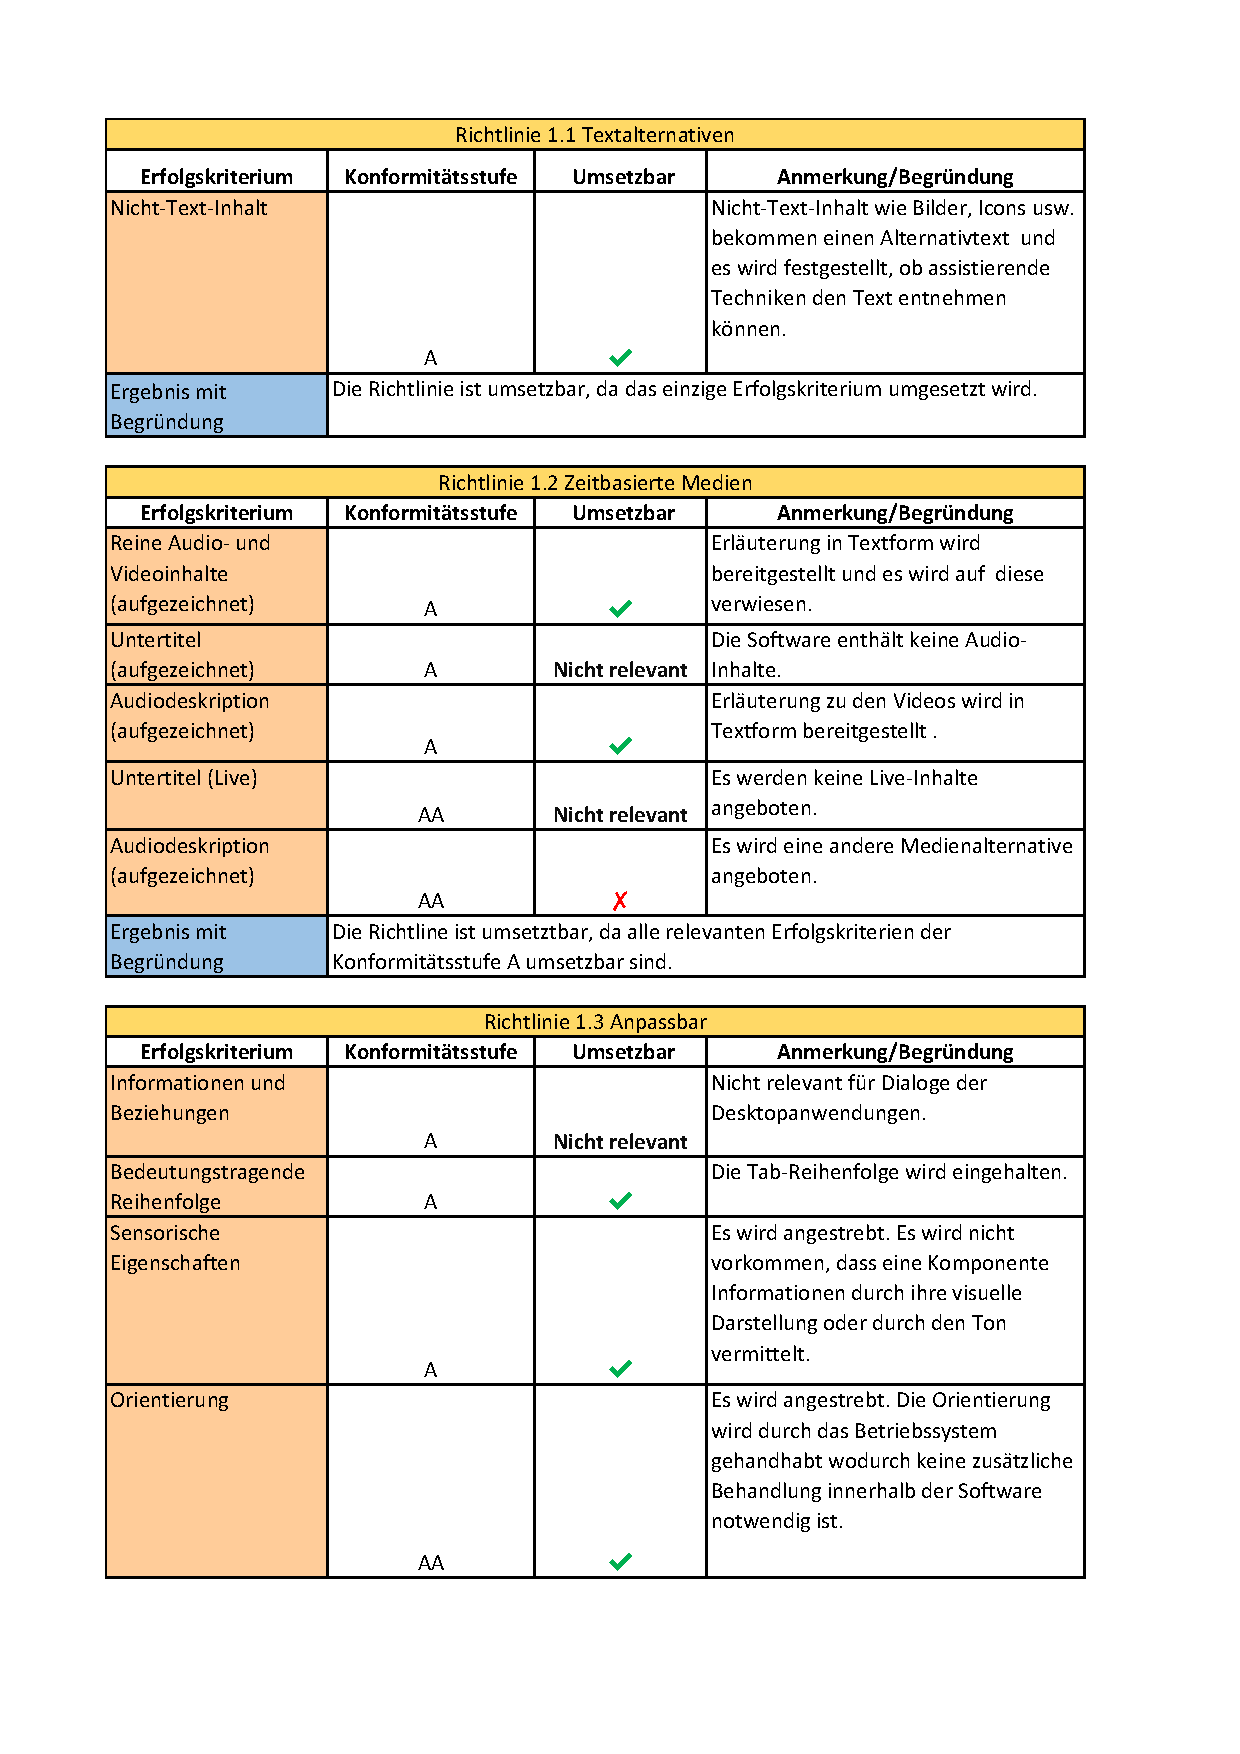
\includepdf[pages=-, scale=0.9, pagecommand={}]{Bewertung der Richtlinien}

\subsubsection{Barrierefreiheit im Software-Entwicklungsprozess}
Beachten die Entwickler die Umsetzung der digitalen Barrierefreiheit von Anfang an nicht, da der Kunde sie im Lastenheft gar nicht verlangt, dann wird eine Umarbeitung der Software sehr aufwendig sein, falls der Kunde sie später doch wünscht.\footnote{Standards für barrierefreie Software \cite{DEVINSIDER}}"`Es empfiehlt sich, bei jeder neuen Entwicklung oder Implementierung, Barrierefreiheit von Anfang an mit zu denken. Zahlreiche Erfahrungen haben gezeigt, dass die Nachrüstung oder Nachbesserung in der Regel deutlich kostenintensiver wird, als die direkte Berücksichtigung."'\footnote{Vgl. Accessibility über Desktopanwendungen hinaus–Barrierefreiheit S. 508 \cite{buhler2017accessibility}}
 
Außerdem ist der Aufwand für das Entwickeln barrierefreier Software von Anfang an geringer als viele Entwickler glauben, da alle  derzeitigen modernen Betriebssysteme globale Funktionen zur Barrierefreiheit anbieten, die der Softwareentwickler dementsprechend nutzen kann, so wie beispielsweise die Bildschirmtastatur, die kontrastreiche Darstellung, die Bildschirmlupe und das Vorlesen von Elementen usw..\footnote{Standards für barrierefreie Software \cite{DEVINSIDER}}

\subsection{Soll-Zustand der Desktopanwendungen}
\label{subsec: Soll-Zustand der Desktopanwendungen}

\comingSoon{+ Die umsetzbare Kriterien werden aufgelistet.\\+ Die Umsetzung erfolgt zu einem späteren Zeitpunkt und nicht in dieser Arbeit.\\+ 4--5 Beispiele für Techniken -> Franz-Josef\\+ Tests werden möglicherweise in einer Folgearbeit betrachtet.}

\section{Fazit \& Ausblick}

\subsection{Zusammenfassung der Arbeit}
Das Thema "`Digitale Barrierefreiheit"' ist seit den 1970er-Jahren eingefordert,\footnote{Accessibility über Desktopanwendungen hinaus–Barrierefreiheit \cite{buhler2017accessibility}} jedoch bekam das Thema seine rechtliche Dimension erst später durch die Normen der \ac{WCAG} sowie der \ac{BITV}. Die digitale Barrierefreiheit umfasst alle digitalen Inhalte, diese können Webseiten, PDFs, Desktopsoftware, Online-Redaktionen, Webkonferenzen, Online-Videos und Mobile-Anwendungen sein. Allerdings ist die Konzentration auf die Webseiten und webbasierte Anwendungen, die meistens digitale Angebote anbieten, stärker. Aus diesem Grund wurde in \cref{subsec: Kriterienvergleich der Barrierefreiheit zwischen Web- und Desktopanwendungen} ein Vergleich zwischen den wesentlichen Eigenschaften der Web- und Desktopanwendungen gezogen und mit dem Ergebnis dieses Vergleiches konnten die Richtlinien der \ac{WCAG} 2.0 bzw. der \ac{WCAG} 2.1 für die Umsetzung in den Desktopanwendungen bewertet werden. Der Nachteil der fehlenden digitalen Barrierefreiheit in jeder Software ist groß, da im schlimmsten Fall nicht nur der Nutzer der Software benachteiligt wird, sondern es werden ganze Zielgruppen ausgeschlossen, was keinem Unternehmen dient. Auf der anderen Seite sind die Vorteile einer barrierefreien Software nicht zu unterschätzen, denn eine barrierefreie Software erreicht mehr Menschen und stellt dem Nutzer keine Hindernisse in den Weg.

\subsection{Erfolgseinschätzung und Ausblick}
Das Ziel dieser Arbeit wurde erreicht, indem die erarbeiteten Kriterien der Standard-Richtlinien der \ac{WCAG} 2.0 bzw. der \ac{WCAG} 2.1 auf die Umsetzung der digitalen Barrierefreiheit in den Desktopanwendungen hin untersucht wurden und damit der Katalog der umsetzbaren Kriterien in \cref{subsec: Soll-Zustand der Desktopanwendungen} erstellt wurde. Für die umsetzbaren Kriterien wurden Maßnahmen in \cref{subsec: Soll-Zustand der Desktopanwendungen} für die Beseitigung der digitalen Barrieren in der aktuellen Software des Unternehmens vorgeschlagen. Diese kommen dementsprechend zum Einsatz in der aktuellen Software und für das Entwickeln neuer Software. Es bleibt jedoch offen, ob die Kriterien, die ausgeschlossen wurden, in der fernen Zukunft zur Anwendungen kommen. Zu einem späteren Zeitpunkt könnten Tools eingesetzt werden, um das Untersuchen der Software auf die Umsetzung der relevanten Kriterien hin zu erleichtern und um sicherzustellen, dass es bei der Umsetzung der Kriterien an nichts fehlt.

% Muss am Ende des Reintexts sein, um die Seitenanzahl davon in Hinweise zum  Umfang der Arbeit zu schreiben
\label{seitenreinschrifft}

%-----------------------------------------------------------

\pagenumbering{Roman}
\setcounter{page}{\value{seitenanzahl}}
\pagestyle{plain.scrheadings}

test 1: \cite{AritcleName}.


\addsec{Quellenverzeichnis}
\printbibliography [heading=none]


\addsec{Anhang}

\subsection*{Anlage 1}
\label{subsec: Anlage1}

\textbf{Allgemeine Grenzwerte zu Blitzen und roten Blitzen (general flash and red flash thresholds)}\footnote{Web Content Accessibility Guidelines 2.0 \cite{WCAG2.0}}

\begin{enumerate}
	\item Ein Blitz oder eine schnell wechselnde Sequenz von Bildern ist unterhalb des Grenzwertes (d.h. Inhalt besteht die Prüfung), wenn eines der Folgenden zutrifft:
	Es gibt nicht mehr als drei allgemeine Blitze und / oder nicht mehr als drei rote Blitze innerhalb von beliebigen Ein-Sekunden-Zeiträumen; oder

	\item Der zusammengenommene Bereich von gleichzeitig auftretenden Blitzen belegt nicht mehr als eine Summe von .006 Steradianten innerhalb jedes beliebigen 10 Grad 		visuellen Feldes auf dem Bildschirm (25\% jedes beliebigen 10-Grad visuellen Feldes auf dem Bildschirm) bei einer typischen Betrachtungsentfernung. Wobei:
	\begin{itemize}
		\item Ein allgemeiner Blitz als ein Paar von entgegengesetzten Änderungen in relativer Luminanz von 10\% oder mehr der maximalen relativen Luminanz definiert wird, 		wobei die relative Luminanz des dunkleren Bildes unter 0.80 liegt; und wo „ein Paar von entgegengesetzten Änderungen“ eine Zunahme gefolgt von einer Abnahme 				ist oder eine Abnahme gefolgt von einer Zunahme. Und
		\item Ein roter Blitz als jedes Paar von entgegengesetzten Übergängen, bei denen ein gesättigtes Rot beteiligt ist, definiert wird.
	\end{itemize}
\end{enumerate}

\textbf{Ausnahme:} Blitzen, das ein feines, ausgeglichenes Muster wie weißes Rauschen oder ein wechselndes Schachbrettmuster mit "`Quadraten"' ist, die auf einer Seite kleiner sind als 0.1 Grad (des visuellen Feldes bei typischem Betrachtungsabstand), verstößt nicht gegen die Grenzwerte.

\textbf{Anmerkung 1:} Die Benutzung eines 341 x 256 Pixel großen Rechtecks irgendwo in dem gezeigten Bildschirmbereich, wenn der Inhalt bei 1024 x 768 Pixeln betrachtet wird, gibt bei allgemeiner Software oder Webinhalten eine gute Einschätzung eines 10 Grad visuellen Feldes für Standard-Bildschirmgrößen und Betrachtungsentfernungen (z.B. 15-17 Zoll Bildschirm bei 56 - 66 cm). (Bildschirme mit höheren Auflösungen, auf denen das gleiche Rendering des Inhalts gezeigt wird, ergeben kleinere und sicherere Bilder, daher werden die geringeren Auflösungen benutzt, um die Grenzwerte zu definieren.)

\textbf{Anmerkung 2:} Ein Übergang ist der Wechsel in relativer Luminanz (oder relativer Luminanz/Farbe für rotes Blitzen) zwischen nebeneinander liegenden Spitzen und Senken in einem Graph von relativer Luminanzmessung (oder relativer Luminanz/Farbe bei rotem Blitzen) in Bezug auf die Zeit. Ein Blitz besteht aus zwei entgegengesetzten Änderungen.

\textbf{Anmerkung 3:} Die derzeitige Arbeitsdefinition in diesem Fachbereich für ein "`Paar von entgegengesetzten Übergängen, die ein gesättigtes Rot beinhalten"' lautet: Wenn für jeden oder beide Zustände, die in jedem Übergang involviert sind, R/(R+ G + B) >= 0.8 und der Wechsel des Wertes von (R-G-B)x320 > 20 (negative Werte von (R-G-B)x320 werden auf Null gesetzt) für beide Übergänge ist. R, G, B Werte reichen von 0-1 wie in der "`relativen Luminanz"'-Definition festgelegt. [HARDING-BINNIE]

\textbf{Anmerkung 4:} Es gibt Werkzeuge, welche die Analyse durch die Erfassung des Video-Bildschirms ausführen. Es ist allerdings kein Werkzeug nötig, um diese Bedingung zu evaluieren, wenn das Blitzen weniger oder gleich 3 Blitze pro Sekunde ist. Der Inhalt besteht automatisch die Prüfung (siehe \# 1 und \# 2 oben).

\appendix


\end{document}
